\documentclass[twoside]{book}

% Packages required by doxygen
\usepackage{calc}
\usepackage{doxygen}
\usepackage{graphicx}
\usepackage[utf8]{inputenc}
\usepackage{makeidx}
\usepackage{multicol}
\usepackage{multirow}
\usepackage{textcomp}
\usepackage[table]{xcolor}

% Font selection
\usepackage[T1]{fontenc}
\usepackage{mathptmx}
\usepackage[scaled=.90]{helvet}
\usepackage{courier}
\usepackage{amssymb}
\usepackage{sectsty}
\renewcommand{\familydefault}{\sfdefault}
\allsectionsfont{%
  \fontseries{bc}\selectfont%
  \color{darkgray}%
}
\renewcommand{\DoxyLabelFont}{%
  \fontseries{bc}\selectfont%
  \color{darkgray}%
}

% Page & text layout
\usepackage{geometry}
\geometry{%
  a4paper,%
  top=2.5cm,%
  bottom=2.5cm,%
  left=2.5cm,%
  right=2.5cm%
}
\tolerance=750
\hfuzz=15pt
\hbadness=750
\setlength{\emergencystretch}{15pt}
\setlength{\parindent}{0cm}
\setlength{\parskip}{0.2cm}
\makeatletter
\renewcommand{\paragraph}{%
  \@startsection{paragraph}{4}{0ex}{-1.0ex}{1.0ex}{%
    \normalfont\normalsize\bfseries\SS@parafont%
  }%
}
\renewcommand{\subparagraph}{%
  \@startsection{subparagraph}{5}{0ex}{-1.0ex}{1.0ex}{%
    \normalfont\normalsize\bfseries\SS@subparafont%
  }%
}
\makeatother

% Headers & footers
\usepackage{fancyhdr}
\pagestyle{fancyplain}
\fancyhead[LE]{\fancyplain{}{\bfseries\thepage}}
\fancyhead[CE]{\fancyplain{}{}}
\fancyhead[RE]{\fancyplain{}{\bfseries\leftmark}}
\fancyhead[LO]{\fancyplain{}{\bfseries\rightmark}}
\fancyhead[CO]{\fancyplain{}{}}
\fancyhead[RO]{\fancyplain{}{\bfseries\thepage}}
\fancyfoot[LE]{\fancyplain{}{}}
\fancyfoot[CE]{\fancyplain{}{}}
\fancyfoot[RE]{\fancyplain{}{\bfseries\scriptsize Generated on Tue May 27 2014 20\-:58\-:30 for Lib Bomberman by Doxygen }}
\fancyfoot[LO]{\fancyplain{}{\bfseries\scriptsize Generated on Tue May 27 2014 20\-:58\-:30 for Lib Bomberman by Doxygen }}
\fancyfoot[CO]{\fancyplain{}{}}
\fancyfoot[RO]{\fancyplain{}{}}
\renewcommand{\footrulewidth}{0.4pt}
\renewcommand{\chaptermark}[1]{%
  \markboth{#1}{}%
}
\renewcommand{\sectionmark}[1]{%
  \markright{\thesection\ #1}%
}

% Indices & bibliography
\usepackage{natbib}
\usepackage[titles]{tocloft}
\setcounter{tocdepth}{3}
\setcounter{secnumdepth}{5}
\makeindex

% Hyperlinks (required, but should be loaded last)
\usepackage{ifpdf}
\ifpdf
  \usepackage[pdftex,pagebackref=true]{hyperref}
\else
  \usepackage[ps2pdf,pagebackref=true]{hyperref}
\fi
\hypersetup{%
  colorlinks=true,%
  linkcolor=blue,%
  citecolor=blue,%
  unicode%
}

% Custom commands
\newcommand{\clearemptydoublepage}{%
  \newpage{\pagestyle{empty}\cleardoublepage}%
}


%===== C O N T E N T S =====

\begin{document}

% Titlepage & ToC
\hypersetup{pageanchor=false}
\pagenumbering{roman}
\begin{titlepage}
\vspace*{7cm}
\begin{center}%
{\Large Lib Bomberman \\[1ex]\large 1.\-0 }\\
\vspace*{1cm}
{\large Generated by Doxygen 1.8.6}\\
\vspace*{0.5cm}
{\small Tue May 27 2014 20:58:30}\\
\end{center}
\end{titlepage}
\clearemptydoublepage
\tableofcontents
\clearemptydoublepage
\pagenumbering{arabic}
\hypersetup{pageanchor=true}

%--- Begin generated contents ---
\chapter{Hierarchical Index}
\section{Class Hierarchy}
This inheritance list is sorted roughly, but not completely, alphabetically\-:\begin{DoxyCompactList}
\item \contentsline{section}{gdl\-:\-:A\-Shader}{\pageref{classgdl_1_1_a_shader}}{}
\begin{DoxyCompactList}
\item \contentsline{section}{gdl\-:\-:Basic\-Shader}{\pageref{classgdl_1_1_basic_shader}}{}
\end{DoxyCompactList}
\item \contentsline{section}{gdl\-:\-:Clock}{\pageref{classgdl_1_1_clock}}{}
\item \contentsline{section}{gdl\-:\-:Game}{\pageref{classgdl_1_1_game}}{}
\item \contentsline{section}{gdl\-:\-:Geometry}{\pageref{classgdl_1_1_geometry}}{}
\item \contentsline{section}{gdl\-:\-:Input}{\pageref{classgdl_1_1_input}}{}
\item \contentsline{section}{gdl\-:\-:I\-Render\-Context}{\pageref{classgdl_1_1_i_render_context}}{}
\begin{DoxyCompactList}
\item \contentsline{section}{gdl\-:\-:Sdl\-Context}{\pageref{classgdl_1_1_sdl_context}}{}
\end{DoxyCompactList}
\item \contentsline{section}{gdl\-:\-:Model}{\pageref{classgdl_1_1_model}}{}
\item \contentsline{section}{gdl\-:\-:Texture}{\pageref{classgdl_1_1_texture}}{}
\end{DoxyCompactList}

\chapter{Class Index}
\section{Class List}
Here are the classes, structs, unions and interfaces with brief descriptions\-:\begin{DoxyCompactList}
\item\contentsline{section}{\hyperlink{classgdl_1_1_a_shader}{gdl\-::\-A\-Shader} \\*This class represents a shader. If you want to create your own shader, you should inherit from this }{\pageref{classgdl_1_1_a_shader}}{}
\item\contentsline{section}{\hyperlink{classgdl_1_1_basic_shader}{gdl\-::\-Basic\-Shader} }{\pageref{classgdl_1_1_basic_shader}}{}
\item\contentsline{section}{\hyperlink{classgdl_1_1_clock}{gdl\-::\-Clock} \\*Class used to get the elapsed time since the last update }{\pageref{classgdl_1_1_clock}}{}
\item\contentsline{section}{\hyperlink{classgdl_1_1_game}{gdl\-::\-Game} \\*It's your job to inherit from this and fill the abstract methods }{\pageref{classgdl_1_1_game}}{}
\item\contentsline{section}{\hyperlink{classgdl_1_1_geometry}{gdl\-::\-Geometry} \\*Class used to create raw geometry by pushing vertex informations }{\pageref{classgdl_1_1_geometry}}{}
\item\contentsline{section}{\hyperlink{classgdl_1_1_input}{gdl\-::\-Input} \\*Handle the user inputs }{\pageref{classgdl_1_1_input}}{}
\item\contentsline{section}{\hyperlink{classgdl_1_1_i_render_context}{gdl\-::\-I\-Render\-Context} \\*Interface for a context }{\pageref{classgdl_1_1_i_render_context}}{}
\item\contentsline{section}{\hyperlink{classgdl_1_1_model}{gdl\-::\-Model} \\*Represents a Fbx, Obj or Collada model }{\pageref{classgdl_1_1_model}}{}
\item\contentsline{section}{\hyperlink{classgdl_1_1_sdl_context}{gdl\-::\-Sdl\-Context} \\*Class for an Sdl Context }{\pageref{classgdl_1_1_sdl_context}}{}
\item\contentsline{section}{\hyperlink{classgdl_1_1_texture}{gdl\-::\-Texture} \\*Class representing an Open\-G\-L texture }{\pageref{classgdl_1_1_texture}}{}
\end{DoxyCompactList}

\chapter{Class Documentation}
\hypertarget{classgdl_1_1_a_shader}{\section{gdl\-:\-:A\-Shader Class Reference}
\label{classgdl_1_1_a_shader}\index{gdl\-::\-A\-Shader@{gdl\-::\-A\-Shader}}
}


This class represents a shader. If you want to create your own shader, you should inherit from this.  




{\ttfamily \#include $<$A\-Shader.\-hh$>$}

Inheritance diagram for gdl\-:\-:A\-Shader\-:\begin{figure}[H]
\begin{center}
\leavevmode
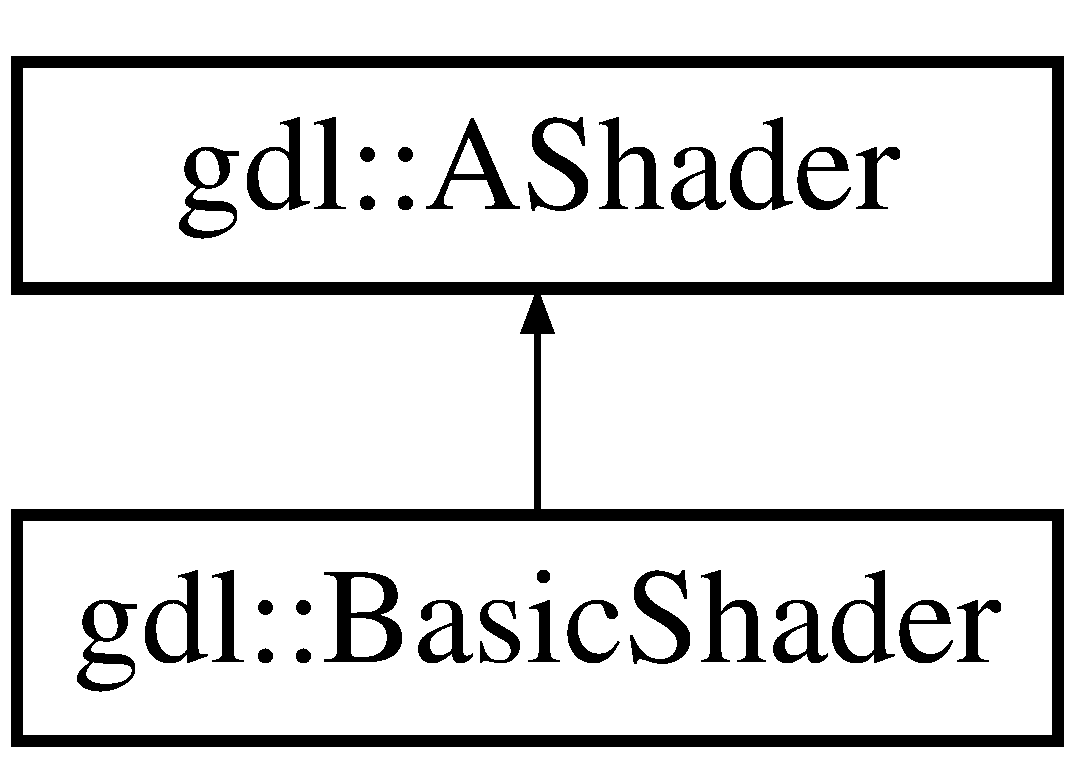
\includegraphics[height=2.000000cm]{classgdl_1_1_a_shader}
\end{center}
\end{figure}
\subsection*{Public Member Functions}
\begin{DoxyCompactItemize}
\item 
\hypertarget{classgdl_1_1_a_shader_a51ce5fd5c2f0afcda913a44ab68ab32b}{void \hyperlink{classgdl_1_1_a_shader_a51ce5fd5c2f0afcda913a44ab68ab32b}{bind} ()}\label{classgdl_1_1_a_shader_a51ce5fd5c2f0afcda913a44ab68ab32b}

\begin{DoxyCompactList}\small\item\em Call gl\-Use\-Program to bind the shader as the current used shader. \end{DoxyCompactList}\item 
G\-Luint \hyperlink{classgdl_1_1_a_shader_af1ed529201e3a16301b3ab0f6d592d54}{get\-Program\-Id} () const 
\begin{DoxyCompactList}\small\item\em Get the program Id. \end{DoxyCompactList}\item 
bool \hyperlink{classgdl_1_1_a_shader_ae292aeb4a9ebf03d2427ba9f44d50136}{load} (const std\-::string \&path, G\-Lenum type)
\begin{DoxyCompactList}\small\item\em Load a vertex or a fragment shader from a file. \end{DoxyCompactList}\item 
G\-Luint \hyperlink{classgdl_1_1_a_shader_a291f4bb70e4374b8a081a57a21e1fe28}{get\-Uniform\-Id} (const std\-::string \&k) const 
\begin{DoxyCompactList}\small\item\em Get the Open\-G\-L location of a constant variable in the shader. \end{DoxyCompactList}\item 
bool \hyperlink{classgdl_1_1_a_shader_ae71efb1e61476a56eb5d4fec32d5d1fa}{set\-Uniform} (const std\-::string \&k, glm\-::vec2 const \&v) const 
\begin{DoxyCompactList}\small\item\em Set a uniform (constant) value in the shader. \end{DoxyCompactList}\item 
bool \hyperlink{classgdl_1_1_a_shader_a4cfe07c7cacb131d08053b2999b3135f}{set\-Uniform} (const std\-::string \&k, glm\-::vec3 const \&v) const 
\begin{DoxyCompactList}\small\item\em Set a uniform (constant) value in the shader. \end{DoxyCompactList}\item 
bool \hyperlink{classgdl_1_1_a_shader_a2ce35c4336139492a98df3db8bdd18d1}{set\-Uniform} (const std\-::string \&k, glm\-::vec4 const \&v) const 
\begin{DoxyCompactList}\small\item\em Set a uniform (constant) value in the shader. \end{DoxyCompactList}\item 
bool \hyperlink{classgdl_1_1_a_shader_a183eb89b2c0f2dc8139c33ff406d7c07}{set\-Uniform} (const std\-::string \&k, glm\-::mat2 const \&v) const 
\begin{DoxyCompactList}\small\item\em Set a uniform (constant) value in the shader. \end{DoxyCompactList}\item 
bool \hyperlink{classgdl_1_1_a_shader_a727f81c327e4662d8ccc9d16d00d500b}{set\-Uniform} (const std\-::string \&k, glm\-::mat3 const \&v) const 
\begin{DoxyCompactList}\small\item\em Set a uniform (constant) value in the shader. \end{DoxyCompactList}\item 
bool \hyperlink{classgdl_1_1_a_shader_a16404bfe7fd48458b5938c1ce280a5b1}{set\-Uniform} (const std\-::string \&k, glm\-::mat4 const \&v) const 
\begin{DoxyCompactList}\small\item\em Set a uniform (constant) value in the shader. \end{DoxyCompactList}\item 
bool \hyperlink{classgdl_1_1_a_shader_abe10dffab7a6b3453281f4cb450b783e}{set\-Uniform} (const std\-::string \&k, glm\-::ivec2 const \&v) const 
\begin{DoxyCompactList}\small\item\em Set a uniform (constant) value in the shader. \end{DoxyCompactList}\item 
bool \hyperlink{classgdl_1_1_a_shader_af0e6f44857b1835c92a0b79606064ab5}{set\-Uniform} (const std\-::string \&k, glm\-::ivec3 const \&v) const 
\begin{DoxyCompactList}\small\item\em Set a uniform (constant) value in the shader. \end{DoxyCompactList}\item 
bool \hyperlink{classgdl_1_1_a_shader_aad8b08fc601c2409b3b670084a1e1a90}{set\-Uniform} (const std\-::string \&k, glm\-::ivec4 const \&v) const 
\begin{DoxyCompactList}\small\item\em Set a uniform (constant) value in the shader. \end{DoxyCompactList}\item 
bool \hyperlink{classgdl_1_1_a_shader_a93d3a6b717cf50326e3c0ca544131845}{set\-Uniform} (const std\-::string \&k, glm\-::uvec2 const \&v) const 
\begin{DoxyCompactList}\small\item\em Set a uniform (constant) value in the shader. \end{DoxyCompactList}\item 
bool \hyperlink{classgdl_1_1_a_shader_a4670bdbe89a3e37d92d035510837465e}{set\-Uniform} (const std\-::string \&k, glm\-::uvec3 const \&v) const 
\begin{DoxyCompactList}\small\item\em Set a uniform (constant) value in the shader. \end{DoxyCompactList}\item 
bool \hyperlink{classgdl_1_1_a_shader_a8b800fb21a0071a28e6093ab99501ae8}{set\-Uniform} (const std\-::string \&k, glm\-::uvec4 const \&v) const 
\begin{DoxyCompactList}\small\item\em Set a uniform (constant) value in the shader. \end{DoxyCompactList}\item 
bool \hyperlink{classgdl_1_1_a_shader_aa166b1e4cd12cf7e157659946861d121}{set\-Uniform} (const std\-::string \&k, float v) const 
\begin{DoxyCompactList}\small\item\em Set a uniform (constant) value in the shader. \end{DoxyCompactList}\item 
bool \hyperlink{classgdl_1_1_a_shader_ad6091e0ccecf8c062e46482d793e0d6c}{set\-Uniform} (const std\-::string \&k, unsigned int v) const 
\begin{DoxyCompactList}\small\item\em Set a uniform (constant) value in the shader. \end{DoxyCompactList}\item 
bool \hyperlink{classgdl_1_1_a_shader_adde4f6da14c5fd786152d81d0a3bb77f}{set\-Uniform} (const std\-::string \&k, int v) const 
\begin{DoxyCompactList}\small\item\em Set a uniform (constant) value in the shader. \end{DoxyCompactList}\item 
bool \hyperlink{classgdl_1_1_a_shader_a882bdda898c0f8a63b3ced52f933e4ef}{set\-Uniform} (const std\-::string \&k, double v) const 
\begin{DoxyCompactList}\small\item\em Set a uniform (constant) value in the shader. \end{DoxyCompactList}\item 
virtual bool \hyperlink{classgdl_1_1_a_shader_a0717c838d5a465332be5b91d12d2dbb5}{build} ()=0
\begin{DoxyCompactList}\small\item\em Build and link the shader (using \-\_\-compile\-Shader and \-\_\-link) and bind the locations of the attributes and samplers. \end{DoxyCompactList}\end{DoxyCompactItemize}
\subsection*{Protected Member Functions}
\begin{DoxyCompactItemize}
\item 
\hypertarget{classgdl_1_1_a_shader_ad0608747a9ef46c049e4bd8960e721d1}{void \hyperlink{classgdl_1_1_a_shader_ad0608747a9ef46c049e4bd8960e721d1}{\-\_\-build} ()}\label{classgdl_1_1_a_shader_ad0608747a9ef46c049e4bd8960e721d1}

\begin{DoxyCompactList}\small\item\em Create the program and attach the shaders loaded This function must be called in the build method after \-\_\-link\-Program. \end{DoxyCompactList}\item 
\hypertarget{classgdl_1_1_a_shader_a791f52f022f2191578b72e3935fb6672}{bool \hyperlink{classgdl_1_1_a_shader_a791f52f022f2191578b72e3935fb6672}{\-\_\-link\-Program} ()}\label{classgdl_1_1_a_shader_a791f52f022f2191578b72e3935fb6672}

\begin{DoxyCompactList}\small\item\em Link the program, This function must be called in the build method just before \-\_\-build. \end{DoxyCompactList}\item 
\hypertarget{classgdl_1_1_a_shader_aeaeb664dec19e428a6e72933e1fc843b}{bool \hyperlink{classgdl_1_1_a_shader_aeaeb664dec19e428a6e72933e1fc843b}{\-\_\-compile\-Shader} (G\-Luint shader\-Id, std\-::string const \&file) const }\label{classgdl_1_1_a_shader_aeaeb664dec19e428a6e72933e1fc843b}

\begin{DoxyCompactList}\small\item\em Compile the shader, This function is called by the load method. \end{DoxyCompactList}\item 
\hypertarget{classgdl_1_1_a_shader_a03c085f34360c4c9e2d5479f88a69916}{void \hyperlink{classgdl_1_1_a_shader_a03c085f34360c4c9e2d5479f88a69916}{\-\_\-bind\-Attrib\-Location} (G\-Luint location, std\-::string const \&attrib\-Name)}\label{classgdl_1_1_a_shader_a03c085f34360c4c9e2d5479f88a69916}

\begin{DoxyCompactList}\small\item\em Bind a shader attribute to a location, This function must be called in the build method before the \-\_\-link\-Program and \-\_\-build. \end{DoxyCompactList}\item 
\hypertarget{classgdl_1_1_a_shader_ad77b6e2c8e74f736bccb2555f35c6fac}{bool \hyperlink{classgdl_1_1_a_shader_ad77b6e2c8e74f736bccb2555f35c6fac}{\-\_\-bind\-Texture\-Unit} (G\-Luint tex\-Unit, std\-::string const \&sampler\-Name)}\label{classgdl_1_1_a_shader_ad77b6e2c8e74f736bccb2555f35c6fac}

\begin{DoxyCompactList}\small\item\em Bind a sampler to the binding point tex\-Unit, This function must be called in the build method after the \-\_\-link\-Program and \-\_\-build. \end{DoxyCompactList}\end{DoxyCompactItemize}


\subsection{Detailed Description}
This class represents a shader. If you want to create your own shader, you should inherit from this. 

\subsection{Member Function Documentation}
\hypertarget{classgdl_1_1_a_shader_a0717c838d5a465332be5b91d12d2dbb5}{\index{gdl\-::\-A\-Shader@{gdl\-::\-A\-Shader}!build@{build}}
\index{build@{build}!gdl::AShader@{gdl\-::\-A\-Shader}}
\subsubsection[{build}]{\setlength{\rightskip}{0pt plus 5cm}virtual bool gdl\-::\-A\-Shader\-::build (
\begin{DoxyParamCaption}
{}
\end{DoxyParamCaption}
)\hspace{0.3cm}{\ttfamily [pure virtual]}}}\label{classgdl_1_1_a_shader_a0717c838d5a465332be5b91d12d2dbb5}


Build and link the shader (using \-\_\-compile\-Shader and \-\_\-link) and bind the locations of the attributes and samplers. 

\begin{DoxyReturn}{Returns}
True if the build succeed, false otherwise. 
\end{DoxyReturn}


Implemented in \hyperlink{classgdl_1_1_basic_shader_a2fbfee8bd2e95b001617bfe34c1e53e4}{gdl\-::\-Basic\-Shader}.

\hypertarget{classgdl_1_1_a_shader_af1ed529201e3a16301b3ab0f6d592d54}{\index{gdl\-::\-A\-Shader@{gdl\-::\-A\-Shader}!get\-Program\-Id@{get\-Program\-Id}}
\index{get\-Program\-Id@{get\-Program\-Id}!gdl::AShader@{gdl\-::\-A\-Shader}}
\subsubsection[{get\-Program\-Id}]{\setlength{\rightskip}{0pt plus 5cm}G\-Luint gdl\-::\-A\-Shader\-::get\-Program\-Id (
\begin{DoxyParamCaption}
{}
\end{DoxyParamCaption}
) const}}\label{classgdl_1_1_a_shader_af1ed529201e3a16301b3ab0f6d592d54}


Get the program Id. 

\begin{DoxyReturn}{Returns}
An unsigned int corresponding to the Open\-G\-L program Id. 
\end{DoxyReturn}
\hypertarget{classgdl_1_1_a_shader_a291f4bb70e4374b8a081a57a21e1fe28}{\index{gdl\-::\-A\-Shader@{gdl\-::\-A\-Shader}!get\-Uniform\-Id@{get\-Uniform\-Id}}
\index{get\-Uniform\-Id@{get\-Uniform\-Id}!gdl::AShader@{gdl\-::\-A\-Shader}}
\subsubsection[{get\-Uniform\-Id}]{\setlength{\rightskip}{0pt plus 5cm}G\-Luint gdl\-::\-A\-Shader\-::get\-Uniform\-Id (
\begin{DoxyParamCaption}
\item[{const std\-::string \&}]{k}
\end{DoxyParamCaption}
) const}}\label{classgdl_1_1_a_shader_a291f4bb70e4374b8a081a57a21e1fe28}


Get the Open\-G\-L location of a constant variable in the shader. 


\begin{DoxyParams}{Parameters}
{\em k} & The uniform variable name. \\
\hline
\end{DoxyParams}
\begin{DoxyReturn}{Returns}
The unsigned int corresponding to the uniform location. 
\end{DoxyReturn}
\hypertarget{classgdl_1_1_a_shader_ae292aeb4a9ebf03d2427ba9f44d50136}{\index{gdl\-::\-A\-Shader@{gdl\-::\-A\-Shader}!load@{load}}
\index{load@{load}!gdl::AShader@{gdl\-::\-A\-Shader}}
\subsubsection[{load}]{\setlength{\rightskip}{0pt plus 5cm}bool gdl\-::\-A\-Shader\-::load (
\begin{DoxyParamCaption}
\item[{const std\-::string \&}]{path, }
\item[{G\-Lenum}]{type}
\end{DoxyParamCaption}
)}}\label{classgdl_1_1_a_shader_ae292aeb4a9ebf03d2427ba9f44d50136}


Load a vertex or a fragment shader from a file. 

\begin{DoxyReturn}{Returns}
A boolean which is false if the load has failed. 
\end{DoxyReturn}

\begin{DoxyParams}{Parameters}
{\em path} & The path to the text file containing the G\-L\-S\-L code. \\
\hline
{\em type} & G\-L\-\_\-\-V\-E\-R\-T\-E\-X\-\_\-\-S\-H\-A\-D\-E\-R, G\-L\-\_\-\-F\-R\-A\-G\-M\-E\-N\-T\-\_\-\-S\-H\-A\-D\-E\-R or G\-L\-\_\-\-G\-E\-O\-M\-E\-T\-R\-Y\-\_\-\-S\-H\-A\-D\-E\-R. \\
\hline
\end{DoxyParams}
\hypertarget{classgdl_1_1_a_shader_ae71efb1e61476a56eb5d4fec32d5d1fa}{\index{gdl\-::\-A\-Shader@{gdl\-::\-A\-Shader}!set\-Uniform@{set\-Uniform}}
\index{set\-Uniform@{set\-Uniform}!gdl::AShader@{gdl\-::\-A\-Shader}}
\subsubsection[{set\-Uniform}]{\setlength{\rightskip}{0pt plus 5cm}bool gdl\-::\-A\-Shader\-::set\-Uniform (
\begin{DoxyParamCaption}
\item[{const std\-::string \&}]{k, }
\item[{glm\-::vec2 const \&}]{v}
\end{DoxyParamCaption}
) const}}\label{classgdl_1_1_a_shader_ae71efb1e61476a56eb5d4fec32d5d1fa}


Set a uniform (constant) value in the shader. 


\begin{DoxyParams}{Parameters}
{\em k} & The name of the uniform variable. \\
\hline
{\em v} & The value of the uniform variable. \\
\hline
\end{DoxyParams}
\begin{DoxyReturn}{Returns}
False if the uniform name is not found in the shader. 
\end{DoxyReturn}
\hypertarget{classgdl_1_1_a_shader_a4cfe07c7cacb131d08053b2999b3135f}{\index{gdl\-::\-A\-Shader@{gdl\-::\-A\-Shader}!set\-Uniform@{set\-Uniform}}
\index{set\-Uniform@{set\-Uniform}!gdl::AShader@{gdl\-::\-A\-Shader}}
\subsubsection[{set\-Uniform}]{\setlength{\rightskip}{0pt plus 5cm}bool gdl\-::\-A\-Shader\-::set\-Uniform (
\begin{DoxyParamCaption}
\item[{const std\-::string \&}]{k, }
\item[{glm\-::vec3 const \&}]{v}
\end{DoxyParamCaption}
) const}}\label{classgdl_1_1_a_shader_a4cfe07c7cacb131d08053b2999b3135f}


Set a uniform (constant) value in the shader. 


\begin{DoxyParams}{Parameters}
{\em k} & The name of the uniform variable. \\
\hline
{\em v} & The value of the uniform variable. \\
\hline
\end{DoxyParams}
\begin{DoxyReturn}{Returns}
False if the uniform name is not found in the shader. 
\end{DoxyReturn}
\hypertarget{classgdl_1_1_a_shader_a2ce35c4336139492a98df3db8bdd18d1}{\index{gdl\-::\-A\-Shader@{gdl\-::\-A\-Shader}!set\-Uniform@{set\-Uniform}}
\index{set\-Uniform@{set\-Uniform}!gdl::AShader@{gdl\-::\-A\-Shader}}
\subsubsection[{set\-Uniform}]{\setlength{\rightskip}{0pt plus 5cm}bool gdl\-::\-A\-Shader\-::set\-Uniform (
\begin{DoxyParamCaption}
\item[{const std\-::string \&}]{k, }
\item[{glm\-::vec4 const \&}]{v}
\end{DoxyParamCaption}
) const}}\label{classgdl_1_1_a_shader_a2ce35c4336139492a98df3db8bdd18d1}


Set a uniform (constant) value in the shader. 


\begin{DoxyParams}{Parameters}
{\em k} & The name of the uniform variable. \\
\hline
{\em v} & The value of the uniform variable. \\
\hline
\end{DoxyParams}
\begin{DoxyReturn}{Returns}
False if the uniform name is not found in the shader. 
\end{DoxyReturn}
\hypertarget{classgdl_1_1_a_shader_a183eb89b2c0f2dc8139c33ff406d7c07}{\index{gdl\-::\-A\-Shader@{gdl\-::\-A\-Shader}!set\-Uniform@{set\-Uniform}}
\index{set\-Uniform@{set\-Uniform}!gdl::AShader@{gdl\-::\-A\-Shader}}
\subsubsection[{set\-Uniform}]{\setlength{\rightskip}{0pt plus 5cm}bool gdl\-::\-A\-Shader\-::set\-Uniform (
\begin{DoxyParamCaption}
\item[{const std\-::string \&}]{k, }
\item[{glm\-::mat2 const \&}]{v}
\end{DoxyParamCaption}
) const}}\label{classgdl_1_1_a_shader_a183eb89b2c0f2dc8139c33ff406d7c07}


Set a uniform (constant) value in the shader. 


\begin{DoxyParams}{Parameters}
{\em k} & The name of the uniform variable. \\
\hline
{\em v} & The value of the uniform variable. \\
\hline
\end{DoxyParams}
\begin{DoxyReturn}{Returns}
False if the uniform name is not found in the shader. 
\end{DoxyReturn}
\hypertarget{classgdl_1_1_a_shader_a727f81c327e4662d8ccc9d16d00d500b}{\index{gdl\-::\-A\-Shader@{gdl\-::\-A\-Shader}!set\-Uniform@{set\-Uniform}}
\index{set\-Uniform@{set\-Uniform}!gdl::AShader@{gdl\-::\-A\-Shader}}
\subsubsection[{set\-Uniform}]{\setlength{\rightskip}{0pt plus 5cm}bool gdl\-::\-A\-Shader\-::set\-Uniform (
\begin{DoxyParamCaption}
\item[{const std\-::string \&}]{k, }
\item[{glm\-::mat3 const \&}]{v}
\end{DoxyParamCaption}
) const}}\label{classgdl_1_1_a_shader_a727f81c327e4662d8ccc9d16d00d500b}


Set a uniform (constant) value in the shader. 


\begin{DoxyParams}{Parameters}
{\em k} & The name of the uniform variable. \\
\hline
{\em v} & The value of the uniform variable. \\
\hline
\end{DoxyParams}
\begin{DoxyReturn}{Returns}
False if the uniform name is not found in the shader. 
\end{DoxyReturn}
\hypertarget{classgdl_1_1_a_shader_a16404bfe7fd48458b5938c1ce280a5b1}{\index{gdl\-::\-A\-Shader@{gdl\-::\-A\-Shader}!set\-Uniform@{set\-Uniform}}
\index{set\-Uniform@{set\-Uniform}!gdl::AShader@{gdl\-::\-A\-Shader}}
\subsubsection[{set\-Uniform}]{\setlength{\rightskip}{0pt plus 5cm}bool gdl\-::\-A\-Shader\-::set\-Uniform (
\begin{DoxyParamCaption}
\item[{const std\-::string \&}]{k, }
\item[{glm\-::mat4 const \&}]{v}
\end{DoxyParamCaption}
) const}}\label{classgdl_1_1_a_shader_a16404bfe7fd48458b5938c1ce280a5b1}


Set a uniform (constant) value in the shader. 


\begin{DoxyParams}{Parameters}
{\em k} & The name of the uniform variable. \\
\hline
{\em v} & The value of the uniform variable. \\
\hline
\end{DoxyParams}
\begin{DoxyReturn}{Returns}
False if the uniform name is not found in the shader. 
\end{DoxyReturn}
\hypertarget{classgdl_1_1_a_shader_abe10dffab7a6b3453281f4cb450b783e}{\index{gdl\-::\-A\-Shader@{gdl\-::\-A\-Shader}!set\-Uniform@{set\-Uniform}}
\index{set\-Uniform@{set\-Uniform}!gdl::AShader@{gdl\-::\-A\-Shader}}
\subsubsection[{set\-Uniform}]{\setlength{\rightskip}{0pt plus 5cm}bool gdl\-::\-A\-Shader\-::set\-Uniform (
\begin{DoxyParamCaption}
\item[{const std\-::string \&}]{k, }
\item[{glm\-::ivec2 const \&}]{v}
\end{DoxyParamCaption}
) const}}\label{classgdl_1_1_a_shader_abe10dffab7a6b3453281f4cb450b783e}


Set a uniform (constant) value in the shader. 


\begin{DoxyParams}{Parameters}
{\em k} & The name of the uniform variable. \\
\hline
{\em v} & The value of the uniform variable. \\
\hline
\end{DoxyParams}
\begin{DoxyReturn}{Returns}
False if the uniform name is not found in the shader. 
\end{DoxyReturn}
\hypertarget{classgdl_1_1_a_shader_af0e6f44857b1835c92a0b79606064ab5}{\index{gdl\-::\-A\-Shader@{gdl\-::\-A\-Shader}!set\-Uniform@{set\-Uniform}}
\index{set\-Uniform@{set\-Uniform}!gdl::AShader@{gdl\-::\-A\-Shader}}
\subsubsection[{set\-Uniform}]{\setlength{\rightskip}{0pt plus 5cm}bool gdl\-::\-A\-Shader\-::set\-Uniform (
\begin{DoxyParamCaption}
\item[{const std\-::string \&}]{k, }
\item[{glm\-::ivec3 const \&}]{v}
\end{DoxyParamCaption}
) const}}\label{classgdl_1_1_a_shader_af0e6f44857b1835c92a0b79606064ab5}


Set a uniform (constant) value in the shader. 


\begin{DoxyParams}{Parameters}
{\em k} & The name of the uniform variable. \\
\hline
{\em v} & The value of the uniform variable. \\
\hline
\end{DoxyParams}
\begin{DoxyReturn}{Returns}
False if the uniform name is not found in the shader. 
\end{DoxyReturn}
\hypertarget{classgdl_1_1_a_shader_aad8b08fc601c2409b3b670084a1e1a90}{\index{gdl\-::\-A\-Shader@{gdl\-::\-A\-Shader}!set\-Uniform@{set\-Uniform}}
\index{set\-Uniform@{set\-Uniform}!gdl::AShader@{gdl\-::\-A\-Shader}}
\subsubsection[{set\-Uniform}]{\setlength{\rightskip}{0pt plus 5cm}bool gdl\-::\-A\-Shader\-::set\-Uniform (
\begin{DoxyParamCaption}
\item[{const std\-::string \&}]{k, }
\item[{glm\-::ivec4 const \&}]{v}
\end{DoxyParamCaption}
) const}}\label{classgdl_1_1_a_shader_aad8b08fc601c2409b3b670084a1e1a90}


Set a uniform (constant) value in the shader. 


\begin{DoxyParams}{Parameters}
{\em k} & The name of the uniform variable. \\
\hline
{\em v} & The value of the uniform variable. \\
\hline
\end{DoxyParams}
\begin{DoxyReturn}{Returns}
False if the uniform name is not found in the shader. 
\end{DoxyReturn}
\hypertarget{classgdl_1_1_a_shader_a93d3a6b717cf50326e3c0ca544131845}{\index{gdl\-::\-A\-Shader@{gdl\-::\-A\-Shader}!set\-Uniform@{set\-Uniform}}
\index{set\-Uniform@{set\-Uniform}!gdl::AShader@{gdl\-::\-A\-Shader}}
\subsubsection[{set\-Uniform}]{\setlength{\rightskip}{0pt plus 5cm}bool gdl\-::\-A\-Shader\-::set\-Uniform (
\begin{DoxyParamCaption}
\item[{const std\-::string \&}]{k, }
\item[{glm\-::uvec2 const \&}]{v}
\end{DoxyParamCaption}
) const}}\label{classgdl_1_1_a_shader_a93d3a6b717cf50326e3c0ca544131845}


Set a uniform (constant) value in the shader. 


\begin{DoxyParams}{Parameters}
{\em k} & The name of the uniform variable. \\
\hline
{\em v} & The value of the uniform variable. \\
\hline
\end{DoxyParams}
\begin{DoxyReturn}{Returns}
False if the uniform name is not found in the shader. 
\end{DoxyReturn}
\hypertarget{classgdl_1_1_a_shader_a4670bdbe89a3e37d92d035510837465e}{\index{gdl\-::\-A\-Shader@{gdl\-::\-A\-Shader}!set\-Uniform@{set\-Uniform}}
\index{set\-Uniform@{set\-Uniform}!gdl::AShader@{gdl\-::\-A\-Shader}}
\subsubsection[{set\-Uniform}]{\setlength{\rightskip}{0pt plus 5cm}bool gdl\-::\-A\-Shader\-::set\-Uniform (
\begin{DoxyParamCaption}
\item[{const std\-::string \&}]{k, }
\item[{glm\-::uvec3 const \&}]{v}
\end{DoxyParamCaption}
) const}}\label{classgdl_1_1_a_shader_a4670bdbe89a3e37d92d035510837465e}


Set a uniform (constant) value in the shader. 


\begin{DoxyParams}{Parameters}
{\em k} & The name of the uniform variable. \\
\hline
{\em v} & The value of the uniform variable. \\
\hline
\end{DoxyParams}
\begin{DoxyReturn}{Returns}
False if the uniform name is not found in the shader. 
\end{DoxyReturn}
\hypertarget{classgdl_1_1_a_shader_a8b800fb21a0071a28e6093ab99501ae8}{\index{gdl\-::\-A\-Shader@{gdl\-::\-A\-Shader}!set\-Uniform@{set\-Uniform}}
\index{set\-Uniform@{set\-Uniform}!gdl::AShader@{gdl\-::\-A\-Shader}}
\subsubsection[{set\-Uniform}]{\setlength{\rightskip}{0pt plus 5cm}bool gdl\-::\-A\-Shader\-::set\-Uniform (
\begin{DoxyParamCaption}
\item[{const std\-::string \&}]{k, }
\item[{glm\-::uvec4 const \&}]{v}
\end{DoxyParamCaption}
) const}}\label{classgdl_1_1_a_shader_a8b800fb21a0071a28e6093ab99501ae8}


Set a uniform (constant) value in the shader. 


\begin{DoxyParams}{Parameters}
{\em k} & The name of the uniform variable. \\
\hline
{\em v} & The value of the uniform variable. \\
\hline
\end{DoxyParams}
\begin{DoxyReturn}{Returns}
False if the uniform name is not found in the shader. 
\end{DoxyReturn}
\hypertarget{classgdl_1_1_a_shader_aa166b1e4cd12cf7e157659946861d121}{\index{gdl\-::\-A\-Shader@{gdl\-::\-A\-Shader}!set\-Uniform@{set\-Uniform}}
\index{set\-Uniform@{set\-Uniform}!gdl::AShader@{gdl\-::\-A\-Shader}}
\subsubsection[{set\-Uniform}]{\setlength{\rightskip}{0pt plus 5cm}bool gdl\-::\-A\-Shader\-::set\-Uniform (
\begin{DoxyParamCaption}
\item[{const std\-::string \&}]{k, }
\item[{float}]{v}
\end{DoxyParamCaption}
) const}}\label{classgdl_1_1_a_shader_aa166b1e4cd12cf7e157659946861d121}


Set a uniform (constant) value in the shader. 


\begin{DoxyParams}{Parameters}
{\em k} & The name of the uniform variable. \\
\hline
{\em v} & The value of the uniform variable. \\
\hline
\end{DoxyParams}
\begin{DoxyReturn}{Returns}
False if the uniform name is not found in the shader. 
\end{DoxyReturn}
\hypertarget{classgdl_1_1_a_shader_ad6091e0ccecf8c062e46482d793e0d6c}{\index{gdl\-::\-A\-Shader@{gdl\-::\-A\-Shader}!set\-Uniform@{set\-Uniform}}
\index{set\-Uniform@{set\-Uniform}!gdl::AShader@{gdl\-::\-A\-Shader}}
\subsubsection[{set\-Uniform}]{\setlength{\rightskip}{0pt plus 5cm}bool gdl\-::\-A\-Shader\-::set\-Uniform (
\begin{DoxyParamCaption}
\item[{const std\-::string \&}]{k, }
\item[{unsigned int}]{v}
\end{DoxyParamCaption}
) const}}\label{classgdl_1_1_a_shader_ad6091e0ccecf8c062e46482d793e0d6c}


Set a uniform (constant) value in the shader. 


\begin{DoxyParams}{Parameters}
{\em k} & The name of the uniform variable. \\
\hline
{\em v} & The value of the uniform variable. \\
\hline
\end{DoxyParams}
\begin{DoxyReturn}{Returns}
False if the uniform name is not found in the shader. 
\end{DoxyReturn}
\hypertarget{classgdl_1_1_a_shader_adde4f6da14c5fd786152d81d0a3bb77f}{\index{gdl\-::\-A\-Shader@{gdl\-::\-A\-Shader}!set\-Uniform@{set\-Uniform}}
\index{set\-Uniform@{set\-Uniform}!gdl::AShader@{gdl\-::\-A\-Shader}}
\subsubsection[{set\-Uniform}]{\setlength{\rightskip}{0pt plus 5cm}bool gdl\-::\-A\-Shader\-::set\-Uniform (
\begin{DoxyParamCaption}
\item[{const std\-::string \&}]{k, }
\item[{int}]{v}
\end{DoxyParamCaption}
) const}}\label{classgdl_1_1_a_shader_adde4f6da14c5fd786152d81d0a3bb77f}


Set a uniform (constant) value in the shader. 


\begin{DoxyParams}{Parameters}
{\em k} & The name of the uniform variable. \\
\hline
{\em v} & The value of the uniform variable. \\
\hline
\end{DoxyParams}
\begin{DoxyReturn}{Returns}
False if the uniform name is not found in the shader. 
\end{DoxyReturn}
\hypertarget{classgdl_1_1_a_shader_a882bdda898c0f8a63b3ced52f933e4ef}{\index{gdl\-::\-A\-Shader@{gdl\-::\-A\-Shader}!set\-Uniform@{set\-Uniform}}
\index{set\-Uniform@{set\-Uniform}!gdl::AShader@{gdl\-::\-A\-Shader}}
\subsubsection[{set\-Uniform}]{\setlength{\rightskip}{0pt plus 5cm}bool gdl\-::\-A\-Shader\-::set\-Uniform (
\begin{DoxyParamCaption}
\item[{const std\-::string \&}]{k, }
\item[{double}]{v}
\end{DoxyParamCaption}
) const}}\label{classgdl_1_1_a_shader_a882bdda898c0f8a63b3ced52f933e4ef}


Set a uniform (constant) value in the shader. 


\begin{DoxyParams}{Parameters}
{\em k} & The name of the uniform variable. \\
\hline
{\em v} & The value of the uniform variable. \\
\hline
\end{DoxyParams}
\begin{DoxyReturn}{Returns}
False if the uniform name is not found in the shader. 
\end{DoxyReturn}


The documentation for this class was generated from the following files\-:\begin{DoxyCompactItemize}
\item 
includes/A\-Shader.\-hh\item 
sources/A\-Shader.\-cpp\end{DoxyCompactItemize}

\hypertarget{classgdl_1_1_basic_shader}{\section{gdl\-:\-:Basic\-Shader Class Reference}
\label{classgdl_1_1_basic_shader}\index{gdl\-::\-Basic\-Shader@{gdl\-::\-Basic\-Shader}}
}
Inheritance diagram for gdl\-:\-:Basic\-Shader\-:\begin{figure}[H]
\begin{center}
\leavevmode
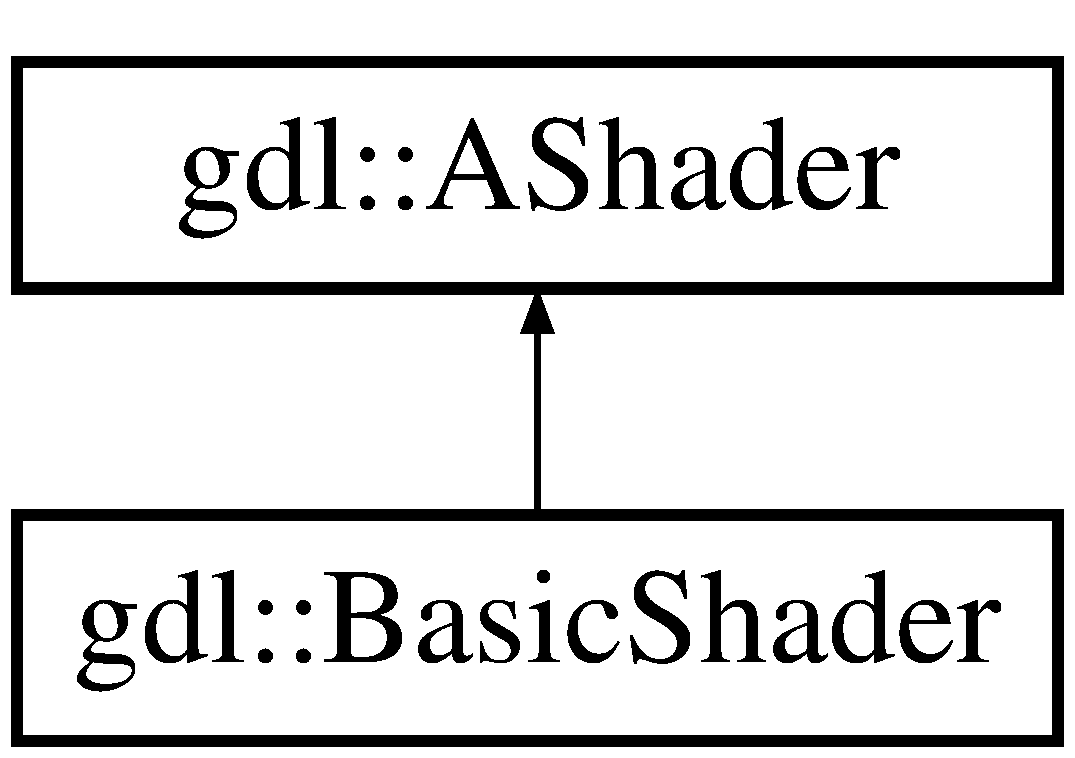
\includegraphics[height=2.000000cm]{classgdl_1_1_basic_shader}
\end{center}
\end{figure}
\subsection*{Public Member Functions}
\begin{DoxyCompactItemize}
\item 
virtual bool \hyperlink{classgdl_1_1_basic_shader_a2fbfee8bd2e95b001617bfe34c1e53e4}{build} ()
\begin{DoxyCompactList}\small\item\em Build and link the shader (using \-\_\-compile\-Shader and \-\_\-link) and bind the locations of the attributes and samplers. \end{DoxyCompactList}\end{DoxyCompactItemize}
\subsection*{Additional Inherited Members}


\subsection{Member Function Documentation}
\hypertarget{classgdl_1_1_basic_shader_a2fbfee8bd2e95b001617bfe34c1e53e4}{\index{gdl\-::\-Basic\-Shader@{gdl\-::\-Basic\-Shader}!build@{build}}
\index{build@{build}!gdl::BasicShader@{gdl\-::\-Basic\-Shader}}
\subsubsection[{build}]{\setlength{\rightskip}{0pt plus 5cm}bool gdl\-::\-Basic\-Shader\-::build (
\begin{DoxyParamCaption}
{}
\end{DoxyParamCaption}
)\hspace{0.3cm}{\ttfamily [virtual]}}}\label{classgdl_1_1_basic_shader_a2fbfee8bd2e95b001617bfe34c1e53e4}


Build and link the shader (using \-\_\-compile\-Shader and \-\_\-link) and bind the locations of the attributes and samplers. 

\begin{DoxyReturn}{Returns}
True if the build succeed, false otherwise. 
\end{DoxyReturn}


Implements \hyperlink{classgdl_1_1_a_shader_a0717c838d5a465332be5b91d12d2dbb5}{gdl\-::\-A\-Shader}.



The documentation for this class was generated from the following files\-:\begin{DoxyCompactItemize}
\item 
includes/Basic\-Shader.\-hh\item 
sources/Basic\-Shader.\-cpp\end{DoxyCompactItemize}

\hypertarget{classgdl_1_1_clock}{\section{gdl\-:\-:Clock Class Reference}
\label{classgdl_1_1_clock}\index{gdl\-::\-Clock@{gdl\-::\-Clock}}
}


Class used to get the elapsed time since the last update.  




{\ttfamily \#include $<$Clock.\-hh$>$}

\subsection*{Public Member Functions}
\begin{DoxyCompactItemize}
\item 
void \hyperlink{classgdl_1_1_clock_a1ec15565cb419cd67e6cdfedf6b112ca}{update} (unsigned int current\-Time)
\begin{DoxyCompactList}\small\item\em Do not call this function yourself! It is used by the context to update the current time. \end{DoxyCompactList}\item 
double \hyperlink{classgdl_1_1_clock_a8ea324bb269ca68e8f5a8c1cf071c3f7}{get\-Elapsed} () const 
\begin{DoxyCompactList}\small\item\em Function used to get the elapsed time since the last update. \end{DoxyCompactList}\end{DoxyCompactItemize}


\subsection{Detailed Description}
Class used to get the elapsed time since the last update. 

\subsection{Member Function Documentation}
\hypertarget{classgdl_1_1_clock_a8ea324bb269ca68e8f5a8c1cf071c3f7}{\index{gdl\-::\-Clock@{gdl\-::\-Clock}!get\-Elapsed@{get\-Elapsed}}
\index{get\-Elapsed@{get\-Elapsed}!gdl::Clock@{gdl\-::\-Clock}}
\subsubsection[{get\-Elapsed}]{\setlength{\rightskip}{0pt plus 5cm}double gdl\-::\-Clock\-::get\-Elapsed (
\begin{DoxyParamCaption}
{}
\end{DoxyParamCaption}
) const}}\label{classgdl_1_1_clock_a8ea324bb269ca68e8f5a8c1cf071c3f7}


Function used to get the elapsed time since the last update. 

\begin{DoxyReturn}{Returns}
The number of seconds elapsed since the last update. 
\end{DoxyReturn}
\hypertarget{classgdl_1_1_clock_a1ec15565cb419cd67e6cdfedf6b112ca}{\index{gdl\-::\-Clock@{gdl\-::\-Clock}!update@{update}}
\index{update@{update}!gdl::Clock@{gdl\-::\-Clock}}
\subsubsection[{update}]{\setlength{\rightskip}{0pt plus 5cm}void gdl\-::\-Clock\-::update (
\begin{DoxyParamCaption}
\item[{unsigned int}]{current\-Time}
\end{DoxyParamCaption}
)}}\label{classgdl_1_1_clock_a1ec15565cb419cd67e6cdfedf6b112ca}


Do not call this function yourself! It is used by the context to update the current time. 


\begin{DoxyParams}{Parameters}
{\em The} & current time in milliseconds. \\
\hline
\end{DoxyParams}


The documentation for this class was generated from the following files\-:\begin{DoxyCompactItemize}
\item 
includes/Clock.\-hh\item 
sources/Clock.\-cpp\end{DoxyCompactItemize}

\hypertarget{classgdl_1_1_game}{\section{gdl\-:\-:Game Class Reference}
\label{classgdl_1_1_game}\index{gdl\-::\-Game@{gdl\-::\-Game}}
}


It's your job to inherit from this and fill the abstract methods.  




{\ttfamily \#include $<$Game.\-hh$>$}

\subsection*{Public Member Functions}
\begin{DoxyCompactItemize}
\item 
\hypertarget{classgdl_1_1_game_aecd7b2ddca26bdea632cd2f7a0dc7b49}{virtual bool \hyperlink{classgdl_1_1_game_aecd7b2ddca26bdea632cd2f7a0dc7b49}{initialize} ()=0}\label{classgdl_1_1_game_aecd7b2ddca26bdea632cd2f7a0dc7b49}

\begin{DoxyCompactList}\small\item\em Pure virtual function used to initialize the game. \end{DoxyCompactList}\item 
\hypertarget{classgdl_1_1_game_a48f421b3d96140732cf028057feca989}{virtual bool \hyperlink{classgdl_1_1_game_a48f421b3d96140732cf028057feca989}{update} ()=0}\label{classgdl_1_1_game_a48f421b3d96140732cf028057feca989}

\begin{DoxyCompactList}\small\item\em Pure virtual function used to update the game logic. \end{DoxyCompactList}\item 
\hypertarget{classgdl_1_1_game_a3de59c743de1fc51cc464f0d47514ffa}{virtual void \hyperlink{classgdl_1_1_game_a3de59c743de1fc51cc464f0d47514ffa}{draw} ()=0}\label{classgdl_1_1_game_a3de59c743de1fc51cc464f0d47514ffa}

\begin{DoxyCompactList}\small\item\em Pure virtual function used to draw a frame. \end{DoxyCompactList}\end{DoxyCompactItemize}


\subsection{Detailed Description}
It's your job to inherit from this and fill the abstract methods. 

The documentation for this class was generated from the following files\-:\begin{DoxyCompactItemize}
\item 
includes/Game.\-hh\item 
sources/Game.\-cpp\end{DoxyCompactItemize}

\hypertarget{classgdl_1_1_geometry}{\section{gdl\-:\-:Geometry Class Reference}
\label{classgdl_1_1_geometry}\index{gdl\-::\-Geometry@{gdl\-::\-Geometry}}
}


Class used to create raw geometry by pushing vertex informations.  




{\ttfamily \#include $<$Geometry.\-hh$>$}

\subsection*{Public Member Functions}
\begin{DoxyCompactItemize}
\item 
\hyperlink{classgdl_1_1_geometry}{Geometry} \& \hyperlink{classgdl_1_1_geometry_afb0537b5e20e5f7aed2621e8fea93f87}{push\-Vertex} (const glm\-::vec3 \&t)
\begin{DoxyCompactList}\small\item\em Push a vertice. \end{DoxyCompactList}\item 
\hyperlink{classgdl_1_1_geometry}{Geometry} \& \hyperlink{classgdl_1_1_geometry_a14d0218f49c1486b9f04de32b6533f1e}{push\-Uv} (const glm\-::vec2 \&t)
\begin{DoxyCompactList}\small\item\em Push a U\-V texture coordinate. \end{DoxyCompactList}\item 
\hyperlink{classgdl_1_1_geometry}{Geometry} \& \hyperlink{classgdl_1_1_geometry_a952a056d62627e002c3516476fd71b99}{push\-Normal} (const glm\-::vec3 \&t)
\begin{DoxyCompactList}\small\item\em Push a normal vector. \end{DoxyCompactList}\item 
\hyperlink{classgdl_1_1_geometry}{Geometry} \& \hyperlink{classgdl_1_1_geometry_abcce9e727917d430e4a68650c50c2a0e}{set\-Color} (const glm\-::vec4 \&t)
\begin{DoxyCompactList}\small\item\em Push a color that is going to be applied on the next pushed vertices. \end{DoxyCompactList}\item 
bool \hyperlink{classgdl_1_1_geometry_a6e8f3c283012d41ea72d4f091b82652d}{build} ()
\begin{DoxyCompactList}\small\item\em Build the current geometry. \end{DoxyCompactList}\item 
void \hyperlink{classgdl_1_1_geometry_a1345bc83eed3ae62fce3158e459e6973}{draw} (\hyperlink{classgdl_1_1_a_shader}{A\-Shader} \&shader, glm\-::mat4 const \&transform, G\-Lenum draw\-Mode)
\begin{DoxyCompactList}\small\item\em Draw the geometry, the build function must have been called before. \end{DoxyCompactList}\end{DoxyCompactItemize}


\subsection{Detailed Description}
Class used to create raw geometry by pushing vertex informations. 

\subsection{Member Function Documentation}
\hypertarget{classgdl_1_1_geometry_a6e8f3c283012d41ea72d4f091b82652d}{\index{gdl\-::\-Geometry@{gdl\-::\-Geometry}!build@{build}}
\index{build@{build}!gdl::Geometry@{gdl\-::\-Geometry}}
\subsubsection[{build}]{\setlength{\rightskip}{0pt plus 5cm}bool gdl\-::\-Geometry\-::build (
\begin{DoxyParamCaption}
{}
\end{DoxyParamCaption}
)}}\label{classgdl_1_1_geometry_a6e8f3c283012d41ea72d4f091b82652d}


Build the current geometry. 

\begin{DoxyReturn}{Returns}
True if the geometry was successfully built, false otherwise. 
\end{DoxyReturn}
\hypertarget{classgdl_1_1_geometry_a1345bc83eed3ae62fce3158e459e6973}{\index{gdl\-::\-Geometry@{gdl\-::\-Geometry}!draw@{draw}}
\index{draw@{draw}!gdl::Geometry@{gdl\-::\-Geometry}}
\subsubsection[{draw}]{\setlength{\rightskip}{0pt plus 5cm}void gdl\-::\-Geometry\-::draw (
\begin{DoxyParamCaption}
\item[{{\bf A\-Shader} \&}]{shader, }
\item[{glm\-::mat4 const \&}]{transform, }
\item[{G\-Lenum}]{draw\-Mode}
\end{DoxyParamCaption}
)}}\label{classgdl_1_1_geometry_a1345bc83eed3ae62fce3158e459e6973}


Draw the geometry, the build function must have been called before. 


\begin{DoxyParams}{Parameters}
{\em shader} & The shader to use for drawing the geometry. \\
\hline
{\em transform} & The model transformation to apply. \\
\hline
{\em dra\-Mode} & The Open\-G\-L draw mode to use (G\-L\-\_\-\-L\-I\-N\-E\-S, G\-L\-\_\-\-T\-R\-I\-A\-N\-G\-L\-E\-S, ...). \\
\hline
\end{DoxyParams}
\hypertarget{classgdl_1_1_geometry_a952a056d62627e002c3516476fd71b99}{\index{gdl\-::\-Geometry@{gdl\-::\-Geometry}!push\-Normal@{push\-Normal}}
\index{push\-Normal@{push\-Normal}!gdl::Geometry@{gdl\-::\-Geometry}}
\subsubsection[{push\-Normal}]{\setlength{\rightskip}{0pt plus 5cm}{\bf Geometry} \& gdl\-::\-Geometry\-::push\-Normal (
\begin{DoxyParamCaption}
\item[{const glm\-::vec3 \&}]{t}
\end{DoxyParamCaption}
)}}\label{classgdl_1_1_geometry_a952a056d62627e002c3516476fd71b99}


Push a normal vector. 


\begin{DoxyParams}{Parameters}
{\em t} & The normal to push. \\
\hline
\end{DoxyParams}
\begin{DoxyReturn}{Returns}
This \hyperlink{classgdl_1_1_geometry}{Geometry}. 
\end{DoxyReturn}
\hypertarget{classgdl_1_1_geometry_a14d0218f49c1486b9f04de32b6533f1e}{\index{gdl\-::\-Geometry@{gdl\-::\-Geometry}!push\-Uv@{push\-Uv}}
\index{push\-Uv@{push\-Uv}!gdl::Geometry@{gdl\-::\-Geometry}}
\subsubsection[{push\-Uv}]{\setlength{\rightskip}{0pt plus 5cm}{\bf Geometry} \& gdl\-::\-Geometry\-::push\-Uv (
\begin{DoxyParamCaption}
\item[{const glm\-::vec2 \&}]{t}
\end{DoxyParamCaption}
)}}\label{classgdl_1_1_geometry_a14d0218f49c1486b9f04de32b6533f1e}


Push a U\-V texture coordinate. 


\begin{DoxyParams}{Parameters}
{\em t} & The U\-V texture coordinate to push. \\
\hline
\end{DoxyParams}
\begin{DoxyReturn}{Returns}
This \hyperlink{classgdl_1_1_geometry}{Geometry}. 
\end{DoxyReturn}
\hypertarget{classgdl_1_1_geometry_afb0537b5e20e5f7aed2621e8fea93f87}{\index{gdl\-::\-Geometry@{gdl\-::\-Geometry}!push\-Vertex@{push\-Vertex}}
\index{push\-Vertex@{push\-Vertex}!gdl::Geometry@{gdl\-::\-Geometry}}
\subsubsection[{push\-Vertex}]{\setlength{\rightskip}{0pt plus 5cm}{\bf Geometry} \& gdl\-::\-Geometry\-::push\-Vertex (
\begin{DoxyParamCaption}
\item[{const glm\-::vec3 \&}]{t}
\end{DoxyParamCaption}
)}}\label{classgdl_1_1_geometry_afb0537b5e20e5f7aed2621e8fea93f87}


Push a vertice. 


\begin{DoxyParams}{Parameters}
{\em t} & The coordinate of the vertice to push. \\
\hline
\end{DoxyParams}
\begin{DoxyReturn}{Returns}
This \hyperlink{classgdl_1_1_geometry}{Geometry}. 
\end{DoxyReturn}
\hypertarget{classgdl_1_1_geometry_abcce9e727917d430e4a68650c50c2a0e}{\index{gdl\-::\-Geometry@{gdl\-::\-Geometry}!set\-Color@{set\-Color}}
\index{set\-Color@{set\-Color}!gdl::Geometry@{gdl\-::\-Geometry}}
\subsubsection[{set\-Color}]{\setlength{\rightskip}{0pt plus 5cm}{\bf Geometry} \& gdl\-::\-Geometry\-::set\-Color (
\begin{DoxyParamCaption}
\item[{const glm\-::vec4 \&}]{t}
\end{DoxyParamCaption}
)}}\label{classgdl_1_1_geometry_abcce9e727917d430e4a68650c50c2a0e}


Push a color that is going to be applied on the next pushed vertices. 


\begin{DoxyParams}{Parameters}
{\em t} & The color to push (rgba). \\
\hline
\end{DoxyParams}
\begin{DoxyReturn}{Returns}
This \hyperlink{classgdl_1_1_geometry}{Geometry}. 
\end{DoxyReturn}


The documentation for this class was generated from the following files\-:\begin{DoxyCompactItemize}
\item 
includes/Geometry.\-hh\item 
sources/Geometry.\-cpp\end{DoxyCompactItemize}

\hypertarget{classgdl_1_1_input}{\section{gdl\-:\-:Input Class Reference}
\label{classgdl_1_1_input}\index{gdl\-::\-Input@{gdl\-::\-Input}}
}


Handle the user inputs.  




{\ttfamily \#include $<$Input.\-hh$>$}

\subsection*{Public Member Functions}
\begin{DoxyCompactItemize}
\item 
\hypertarget{classgdl_1_1_input_a2cbd704d4c1069ac1fd7c4fb91d30b09}{void \hyperlink{classgdl_1_1_input_a2cbd704d4c1069ac1fd7c4fb91d30b09}{clear\-Inputs} ()}\label{classgdl_1_1_input_a2cbd704d4c1069ac1fd7c4fb91d30b09}

\begin{DoxyCompactList}\small\item\em Clear the input list. /!\textbackslash{} Do not call this function. \end{DoxyCompactList}\item 
void \hyperlink{classgdl_1_1_input_a7a175a63e780f1aa0fdebba68c0e8850}{add\-Input} (int input)
\begin{DoxyCompactList}\small\item\em Add an input. /!\textbackslash{} Do not call this function. \end{DoxyCompactList}\item 
void \hyperlink{classgdl_1_1_input_aa3380058a91f20b4889371ea07fd2bb4}{add\-Key\-Input} (int input)
\begin{DoxyCompactList}\small\item\em Add a key input. /!\textbackslash{} Do not call this function. \end{DoxyCompactList}\item 
void \hyperlink{classgdl_1_1_input_a531d2a805f5fdd33a0ce70ad74d0b3f8}{remove\-Key\-Input} (int input)
\begin{DoxyCompactList}\small\item\em Remove a key input from the list. /!\textbackslash{} Do not call this function. \end{DoxyCompactList}\item 
void \hyperlink{classgdl_1_1_input_aa6be10489840280271415ec1311ce5af}{set\-Mouse\-Position} (glm\-::ivec2 const \&pos, glm\-::ivec2 const \&rel)
\begin{DoxyCompactList}\small\item\em Set the current mouse position. /!\textbackslash{} Do not call this function. \end{DoxyCompactList}\item 
void \hyperlink{classgdl_1_1_input_a4864b681a18a087443024160861587fb}{set\-Mouse\-Wheel} (glm\-::ivec2 const \&delta)
\begin{DoxyCompactList}\small\item\em Set the current mouse wheel delta. /!\textbackslash{} Do not call this function. \end{DoxyCompactList}\item 
glm\-::ivec2 const \& \hyperlink{classgdl_1_1_input_afa2d25f94d2223a056be6fb5bcda935b}{get\-Mouse\-Position} ()
\begin{DoxyCompactList}\small\item\em Get the mouse position in pixels. \end{DoxyCompactList}\item 
glm\-::ivec2 const \& \hyperlink{classgdl_1_1_input_acf028a2fe8c45c19f6cf4145aeacc400}{get\-Mouse\-Delta} ()
\begin{DoxyCompactList}\small\item\em Get the mouse movement since the last update. \end{DoxyCompactList}\item 
glm\-::ivec2 const \& \hyperlink{classgdl_1_1_input_aaf79c0499e88cfabe234eb894a8122f2}{get\-Mouse\-Wheel} ()
\begin{DoxyCompactList}\small\item\em Get the mouse wheel movement since the last update. \end{DoxyCompactList}\item 
bool \hyperlink{classgdl_1_1_input_a7d26a492aaf056166fe64ec00a927b7a}{get\-Input} (int input, bool handled=false)
\begin{DoxyCompactList}\small\item\em Check if an input is currently happening. \end{DoxyCompactList}\item 
bool \hyperlink{classgdl_1_1_input_a8edd2ea49ebf6c8a833a65cf80133c4c}{get\-Key} (int input, bool handled=false)
\begin{DoxyCompactList}\small\item\em Check if an input is currently happening. \end{DoxyCompactList}\end{DoxyCompactItemize}


\subsection{Detailed Description}
Handle the user inputs. 

\subsection{Member Function Documentation}
\hypertarget{classgdl_1_1_input_a7a175a63e780f1aa0fdebba68c0e8850}{\index{gdl\-::\-Input@{gdl\-::\-Input}!add\-Input@{add\-Input}}
\index{add\-Input@{add\-Input}!gdl::Input@{gdl\-::\-Input}}
\subsubsection[{add\-Input}]{\setlength{\rightskip}{0pt plus 5cm}void gdl\-::\-Input\-::add\-Input (
\begin{DoxyParamCaption}
\item[{int}]{input}
\end{DoxyParamCaption}
)}}\label{classgdl_1_1_input_a7a175a63e780f1aa0fdebba68c0e8850}


Add an input. /!\textbackslash{} Do not call this function. 


\begin{DoxyParams}{Parameters}
{\em input} & The input to add. \\
\hline
\end{DoxyParams}
\hypertarget{classgdl_1_1_input_aa3380058a91f20b4889371ea07fd2bb4}{\index{gdl\-::\-Input@{gdl\-::\-Input}!add\-Key\-Input@{add\-Key\-Input}}
\index{add\-Key\-Input@{add\-Key\-Input}!gdl::Input@{gdl\-::\-Input}}
\subsubsection[{add\-Key\-Input}]{\setlength{\rightskip}{0pt plus 5cm}void gdl\-::\-Input\-::add\-Key\-Input (
\begin{DoxyParamCaption}
\item[{int}]{input}
\end{DoxyParamCaption}
)}}\label{classgdl_1_1_input_aa3380058a91f20b4889371ea07fd2bb4}


Add a key input. /!\textbackslash{} Do not call this function. 


\begin{DoxyParams}{Parameters}
{\em input} & The key to add. \\
\hline
\end{DoxyParams}
\hypertarget{classgdl_1_1_input_a7d26a492aaf056166fe64ec00a927b7a}{\index{gdl\-::\-Input@{gdl\-::\-Input}!get\-Input@{get\-Input}}
\index{get\-Input@{get\-Input}!gdl::Input@{gdl\-::\-Input}}
\subsubsection[{get\-Input}]{\setlength{\rightskip}{0pt plus 5cm}bool gdl\-::\-Input\-::get\-Input (
\begin{DoxyParamCaption}
\item[{int}]{input, }
\item[{bool}]{handled = {\ttfamily false}}
\end{DoxyParamCaption}
)}}\label{classgdl_1_1_input_a7d26a492aaf056166fe64ec00a927b7a}


Check if an input is currently happening. 


\begin{DoxyParams}{Parameters}
{\em input} & The input to check (For an \hyperlink{classgdl_1_1_sdl_context}{Sdl\-Context}, it will be S\-D\-L\-\_\-\-Q\-U\-I\-T, ...). \\
\hline
{\em handled} & If true, remove the input from the list and this function will not return true for this input anymore until the next update. \\
\hline
\end{DoxyParams}
\begin{DoxyReturn}{Returns}
True if the input passed as parameter has been detected. 
\end{DoxyReturn}
\hypertarget{classgdl_1_1_input_a8edd2ea49ebf6c8a833a65cf80133c4c}{\index{gdl\-::\-Input@{gdl\-::\-Input}!get\-Key@{get\-Key}}
\index{get\-Key@{get\-Key}!gdl::Input@{gdl\-::\-Input}}
\subsubsection[{get\-Key}]{\setlength{\rightskip}{0pt plus 5cm}bool gdl\-::\-Input\-::get\-Key (
\begin{DoxyParamCaption}
\item[{int}]{input, }
\item[{bool}]{handled = {\ttfamily false}}
\end{DoxyParamCaption}
)}}\label{classgdl_1_1_input_a8edd2ea49ebf6c8a833a65cf80133c4c}


Check if an input is currently happening. 


\begin{DoxyParams}{Parameters}
{\em input} & The key input to check (For an \hyperlink{classgdl_1_1_sdl_context}{Sdl\-Context}, it will be S\-D\-L\-K\-\_\-\-U\-P, S\-D\-L\-K\-\_\-a, ...). \\
\hline
{\em handled} & If true, remove the input from the list and this function will not return true for this input anymore until the next update. \\
\hline
\end{DoxyParams}
\begin{DoxyReturn}{Returns}
True if the input passed as parameter has been detected. 
\end{DoxyReturn}
\hypertarget{classgdl_1_1_input_acf028a2fe8c45c19f6cf4145aeacc400}{\index{gdl\-::\-Input@{gdl\-::\-Input}!get\-Mouse\-Delta@{get\-Mouse\-Delta}}
\index{get\-Mouse\-Delta@{get\-Mouse\-Delta}!gdl::Input@{gdl\-::\-Input}}
\subsubsection[{get\-Mouse\-Delta}]{\setlength{\rightskip}{0pt plus 5cm}glm\-::ivec2 const \& gdl\-::\-Input\-::get\-Mouse\-Delta (
\begin{DoxyParamCaption}
{}
\end{DoxyParamCaption}
)}}\label{classgdl_1_1_input_acf028a2fe8c45c19f6cf4145aeacc400}


Get the mouse movement since the last update. 

\begin{DoxyReturn}{Returns}
The mouse delta in pixels. 
\end{DoxyReturn}
\hypertarget{classgdl_1_1_input_afa2d25f94d2223a056be6fb5bcda935b}{\index{gdl\-::\-Input@{gdl\-::\-Input}!get\-Mouse\-Position@{get\-Mouse\-Position}}
\index{get\-Mouse\-Position@{get\-Mouse\-Position}!gdl::Input@{gdl\-::\-Input}}
\subsubsection[{get\-Mouse\-Position}]{\setlength{\rightskip}{0pt plus 5cm}glm\-::ivec2 const \& gdl\-::\-Input\-::get\-Mouse\-Position (
\begin{DoxyParamCaption}
{}
\end{DoxyParamCaption}
)}}\label{classgdl_1_1_input_afa2d25f94d2223a056be6fb5bcda935b}


Get the mouse position in pixels. 

\begin{DoxyReturn}{Returns}
The mouse position. 
\end{DoxyReturn}
\hypertarget{classgdl_1_1_input_aaf79c0499e88cfabe234eb894a8122f2}{\index{gdl\-::\-Input@{gdl\-::\-Input}!get\-Mouse\-Wheel@{get\-Mouse\-Wheel}}
\index{get\-Mouse\-Wheel@{get\-Mouse\-Wheel}!gdl::Input@{gdl\-::\-Input}}
\subsubsection[{get\-Mouse\-Wheel}]{\setlength{\rightskip}{0pt plus 5cm}glm\-::ivec2 const \& gdl\-::\-Input\-::get\-Mouse\-Wheel (
\begin{DoxyParamCaption}
{}
\end{DoxyParamCaption}
)}}\label{classgdl_1_1_input_aaf79c0499e88cfabe234eb894a8122f2}


Get the mouse wheel movement since the last update. 

\begin{DoxyReturn}{Returns}
The mouse wheel delta in pixels. 
\end{DoxyReturn}
\hypertarget{classgdl_1_1_input_a531d2a805f5fdd33a0ce70ad74d0b3f8}{\index{gdl\-::\-Input@{gdl\-::\-Input}!remove\-Key\-Input@{remove\-Key\-Input}}
\index{remove\-Key\-Input@{remove\-Key\-Input}!gdl::Input@{gdl\-::\-Input}}
\subsubsection[{remove\-Key\-Input}]{\setlength{\rightskip}{0pt plus 5cm}void gdl\-::\-Input\-::remove\-Key\-Input (
\begin{DoxyParamCaption}
\item[{int}]{input}
\end{DoxyParamCaption}
)}}\label{classgdl_1_1_input_a531d2a805f5fdd33a0ce70ad74d0b3f8}


Remove a key input from the list. /!\textbackslash{} Do not call this function. 


\begin{DoxyParams}{Parameters}
{\em input} & The key input to remove \\
\hline
\end{DoxyParams}
\hypertarget{classgdl_1_1_input_aa6be10489840280271415ec1311ce5af}{\index{gdl\-::\-Input@{gdl\-::\-Input}!set\-Mouse\-Position@{set\-Mouse\-Position}}
\index{set\-Mouse\-Position@{set\-Mouse\-Position}!gdl::Input@{gdl\-::\-Input}}
\subsubsection[{set\-Mouse\-Position}]{\setlength{\rightskip}{0pt plus 5cm}void gdl\-::\-Input\-::set\-Mouse\-Position (
\begin{DoxyParamCaption}
\item[{glm\-::ivec2 const \&}]{pos, }
\item[{glm\-::ivec2 const \&}]{rel}
\end{DoxyParamCaption}
)}}\label{classgdl_1_1_input_aa6be10489840280271415ec1311ce5af}


Set the current mouse position. /!\textbackslash{} Do not call this function. 


\begin{DoxyParams}{Parameters}
{\em pos} & The current mouse position. \\
\hline
{\em rel} & The offset since the last mouse position. \\
\hline
\end{DoxyParams}
\hypertarget{classgdl_1_1_input_a4864b681a18a087443024160861587fb}{\index{gdl\-::\-Input@{gdl\-::\-Input}!set\-Mouse\-Wheel@{set\-Mouse\-Wheel}}
\index{set\-Mouse\-Wheel@{set\-Mouse\-Wheel}!gdl::Input@{gdl\-::\-Input}}
\subsubsection[{set\-Mouse\-Wheel}]{\setlength{\rightskip}{0pt plus 5cm}void gdl\-::\-Input\-::set\-Mouse\-Wheel (
\begin{DoxyParamCaption}
\item[{glm\-::ivec2 const \&}]{delta}
\end{DoxyParamCaption}
)}}\label{classgdl_1_1_input_a4864b681a18a087443024160861587fb}


Set the current mouse wheel delta. /!\textbackslash{} Do not call this function. 


\begin{DoxyParams}{Parameters}
{\em delta} & The current mouse wheel delta. \\
\hline
\end{DoxyParams}


The documentation for this class was generated from the following files\-:\begin{DoxyCompactItemize}
\item 
includes/Input.\-hh\item 
sources/Input.\-cpp\end{DoxyCompactItemize}

\hypertarget{classgdl_1_1_i_render_context}{\section{gdl\-:\-:I\-Render\-Context Class Reference}
\label{classgdl_1_1_i_render_context}\index{gdl\-::\-I\-Render\-Context@{gdl\-::\-I\-Render\-Context}}
}


Interface for a context.  




{\ttfamily \#include $<$I\-Render\-Context.\-hh$>$}

Inheritance diagram for gdl\-:\-:I\-Render\-Context\-:\begin{figure}[H]
\begin{center}
\leavevmode
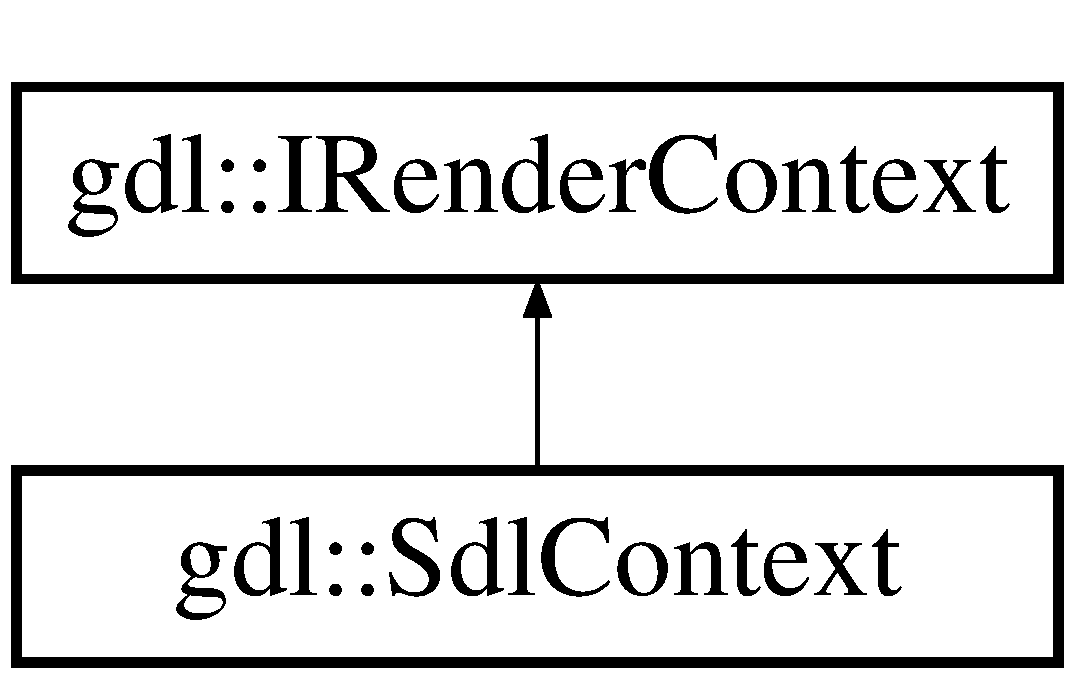
\includegraphics[height=2.000000cm]{classgdl_1_1_i_render_context}
\end{center}
\end{figure}
\subsection*{Public Member Functions}
\begin{DoxyCompactItemize}
\item 
\hypertarget{classgdl_1_1_i_render_context_a962fd24dc84758aaa7c7d28330c3e37e}{virtual bool {\bfseries start} (unsigned int swidth, unsigned int sheight, const std\-::string \&name, int init\-Flags, int windows\-Flags)=0}\label{classgdl_1_1_i_render_context_a962fd24dc84758aaa7c7d28330c3e37e}

\item 
\hypertarget{classgdl_1_1_i_render_context_a19ffcdcc82d88098693a08f66beab770}{virtual void {\bfseries update\-Inputs} (\hyperlink{classgdl_1_1_input}{Input} \&input) const =0}\label{classgdl_1_1_i_render_context_a19ffcdcc82d88098693a08f66beab770}

\item 
\hypertarget{classgdl_1_1_i_render_context_af2134a929634632ccf13e779f489cdc2}{virtual void {\bfseries update\-Clock} (\hyperlink{classgdl_1_1_clock}{Clock} \&clock) const =0}\label{classgdl_1_1_i_render_context_af2134a929634632ccf13e779f489cdc2}

\item 
\hypertarget{classgdl_1_1_i_render_context_aa7ad85ff39d1e82f25162b71284b3659}{virtual void {\bfseries flush} () const =0}\label{classgdl_1_1_i_render_context_aa7ad85ff39d1e82f25162b71284b3659}

\item 
\hypertarget{classgdl_1_1_i_render_context_af1f487e928504f86f878f904fb4075cf}{virtual void {\bfseries stop} () const =0}\label{classgdl_1_1_i_render_context_af1f487e928504f86f878f904fb4075cf}

\end{DoxyCompactItemize}


\subsection{Detailed Description}
Interface for a context. 

The documentation for this class was generated from the following file\-:\begin{DoxyCompactItemize}
\item 
includes/I\-Render\-Context.\-hh\end{DoxyCompactItemize}

\hypertarget{classgdl_1_1_model}{\section{gdl\-:\-:Model Class Reference}
\label{classgdl_1_1_model}\index{gdl\-::\-Model@{gdl\-::\-Model}}
}


Represents a Fbx, Obj or Collada model.  




{\ttfamily \#include $<$Model.\-hh$>$}

\subsection*{Public Member Functions}
\begin{DoxyCompactItemize}
\item 
void \hyperlink{classgdl_1_1_model_a2880a8151a0a076dccc17c8a12530dcc}{pause} (bool pause\-Anim)
\begin{DoxyCompactList}\small\item\em set the pause state for the current animation. \end{DoxyCompactList}\item 
bool \hyperlink{classgdl_1_1_model_a223b04dc9a2007ac22cc71d019af5749}{set\-Current\-Anim} (int stack, bool loop=true)
\begin{DoxyCompactList}\small\item\em Set the current animation by it's index. \end{DoxyCompactList}\item 
bool \hyperlink{classgdl_1_1_model_ac4210edf1cfc619f8948e83820b41ca9}{set\-Current\-Anim} (std\-::string const \&name, bool loop=true)
\begin{DoxyCompactList}\small\item\em Set the current animation by it's name. \end{DoxyCompactList}\item 
int \hyperlink{classgdl_1_1_model_a6c07ff9af9e5f21976f74c76969c5209}{get\-Animation\-Frame\-Number} (int stack)
\begin{DoxyCompactList}\small\item\em Get the number of frame of an animation. \end{DoxyCompactList}\item 
int \hyperlink{classgdl_1_1_model_a2f46e23c1f5bbf46724ab88d4e09edeb}{get\-Animation\-Frame\-Number} (std\-::string const \&name)
\begin{DoxyCompactList}\small\item\em Get the number of frame of an animation. \end{DoxyCompactList}\item 
float \hyperlink{classgdl_1_1_model_a145f9bb956d043c28f23d8714e72447c}{get\-Frame\-Duration} ()
\begin{DoxyCompactList}\small\item\em Get the time of one animation frame. \end{DoxyCompactList}\item 
bool \hyperlink{classgdl_1_1_model_ac903e3a9a4da067bf245a26e4bb02fd0}{create\-Sub\-Anim} (int stack, std\-::string const \&sub\-Anim\-Name, int frame\-Start, int frame\-End)
\begin{DoxyCompactList}\small\item\em Create a sub animation depending on the name or index of a model animation. \end{DoxyCompactList}\item 
bool \hyperlink{classgdl_1_1_model_aa712f9125986a0d0ee9520e73a2a0f66}{create\-Sub\-Anim} (std\-::string const \&name, std\-::string const \&sub\-Anim\-Name, int frame\-Start, int frame\-End)
\begin{DoxyCompactList}\small\item\em Create a sub animation depending on the name or index of a model animation. \end{DoxyCompactList}\item 
bool \hyperlink{classgdl_1_1_model_a7167ca64cd426f7bd46756ed33bad12f}{set\-Current\-Sub\-Anim} (std\-::string const \&name, bool loop=true)
\begin{DoxyCompactList}\small\item\em Set the current sub animation to play. \end{DoxyCompactList}\item 
bool \hyperlink{classgdl_1_1_model_a73175b246228b1a275a4cf2b59c8d5cd}{load} (std\-::string const \&path)
\begin{DoxyCompactList}\small\item\em Load an Fbx, Obj or collada model. \end{DoxyCompactList}\item 
void \hyperlink{classgdl_1_1_model_a57be549452c2bef282709fe02b0072a3}{draw} (\hyperlink{classgdl_1_1_a_shader}{A\-Shader} \&shader, glm\-::mat4 const \&transform, double delta\-Time)
\begin{DoxyCompactList}\small\item\em Draw the current model and update its animation. \end{DoxyCompactList}\end{DoxyCompactItemize}


\subsection{Detailed Description}
Represents a Fbx, Obj or Collada model. 

\subsection{Member Function Documentation}
\hypertarget{classgdl_1_1_model_ac903e3a9a4da067bf245a26e4bb02fd0}{\index{gdl\-::\-Model@{gdl\-::\-Model}!create\-Sub\-Anim@{create\-Sub\-Anim}}
\index{create\-Sub\-Anim@{create\-Sub\-Anim}!gdl::Model@{gdl\-::\-Model}}
\subsubsection[{create\-Sub\-Anim}]{\setlength{\rightskip}{0pt plus 5cm}bool gdl\-::\-Model\-::create\-Sub\-Anim (
\begin{DoxyParamCaption}
\item[{int}]{stack, }
\item[{std\-::string const \&}]{sub\-Anim\-Name, }
\item[{int}]{frame\-Start, }
\item[{int}]{frame\-End}
\end{DoxyParamCaption}
)}}\label{classgdl_1_1_model_ac903e3a9a4da067bf245a26e4bb02fd0}


Create a sub animation depending on the name or index of a model animation. 


\begin{DoxyParams}{Parameters}
{\em stack} & The index of the animation to cut. \\
\hline
{\em sub\-Anim\-Name} & The name of the sub animation to create. \\
\hline
{\em frame\-Start} & The index of the first sub animation frame. \\
\hline
{\em frame\-End} & The index of the last sub animation frame. \\
\hline
\end{DoxyParams}
\begin{DoxyReturn}{Returns}
True if the creation of the sub animation has worked, false otherwise. 
\end{DoxyReturn}
\hypertarget{classgdl_1_1_model_aa712f9125986a0d0ee9520e73a2a0f66}{\index{gdl\-::\-Model@{gdl\-::\-Model}!create\-Sub\-Anim@{create\-Sub\-Anim}}
\index{create\-Sub\-Anim@{create\-Sub\-Anim}!gdl::Model@{gdl\-::\-Model}}
\subsubsection[{create\-Sub\-Anim}]{\setlength{\rightskip}{0pt plus 5cm}bool gdl\-::\-Model\-::create\-Sub\-Anim (
\begin{DoxyParamCaption}
\item[{std\-::string const \&}]{name, }
\item[{std\-::string const \&}]{sub\-Anim\-Name, }
\item[{int}]{frame\-Start, }
\item[{int}]{frame\-End}
\end{DoxyParamCaption}
)}}\label{classgdl_1_1_model_aa712f9125986a0d0ee9520e73a2a0f66}


Create a sub animation depending on the name or index of a model animation. 


\begin{DoxyParams}{Parameters}
{\em stack} & The name of the animation to cut. \\
\hline
{\em sub\-Anim\-Name} & The name of the sub animation to create. \\
\hline
{\em frame\-Start} & The index of the first sub animation frame. \\
\hline
{\em frame\-End} & The index of the last sub animation frame. \\
\hline
\end{DoxyParams}
\begin{DoxyReturn}{Returns}
True if the creation of the sub animation has worked, false otherwise. 
\end{DoxyReturn}
\hypertarget{classgdl_1_1_model_a57be549452c2bef282709fe02b0072a3}{\index{gdl\-::\-Model@{gdl\-::\-Model}!draw@{draw}}
\index{draw@{draw}!gdl::Model@{gdl\-::\-Model}}
\subsubsection[{draw}]{\setlength{\rightskip}{0pt plus 5cm}void gdl\-::\-Model\-::draw (
\begin{DoxyParamCaption}
\item[{{\bf A\-Shader} \&}]{shader, }
\item[{glm\-::mat4 const \&}]{transform, }
\item[{double}]{delta\-Time}
\end{DoxyParamCaption}
)}}\label{classgdl_1_1_model_a57be549452c2bef282709fe02b0072a3}


Draw the current model and update its animation. 


\begin{DoxyParams}{Parameters}
{\em shader} & The shader with which the model will be drawn \\
\hline
{\em transform} & The transformation of the model. \\
\hline
{\em delta\-Time} & The time elapsed since the last frame in seconds (if you want to update the animation). \\
\hline
\end{DoxyParams}
\hypertarget{classgdl_1_1_model_a6c07ff9af9e5f21976f74c76969c5209}{\index{gdl\-::\-Model@{gdl\-::\-Model}!get\-Animation\-Frame\-Number@{get\-Animation\-Frame\-Number}}
\index{get\-Animation\-Frame\-Number@{get\-Animation\-Frame\-Number}!gdl::Model@{gdl\-::\-Model}}
\subsubsection[{get\-Animation\-Frame\-Number}]{\setlength{\rightskip}{0pt plus 5cm}int gdl\-::\-Model\-::get\-Animation\-Frame\-Number (
\begin{DoxyParamCaption}
\item[{int}]{stack}
\end{DoxyParamCaption}
)}}\label{classgdl_1_1_model_a6c07ff9af9e5f21976f74c76969c5209}


Get the number of frame of an animation. 


\begin{DoxyParams}{Parameters}
{\em stack} & The index of the animation. \\
\hline
\end{DoxyParams}
\begin{DoxyReturn}{Returns}
The number of frame in this animation. 
\end{DoxyReturn}
\hypertarget{classgdl_1_1_model_a2f46e23c1f5bbf46724ab88d4e09edeb}{\index{gdl\-::\-Model@{gdl\-::\-Model}!get\-Animation\-Frame\-Number@{get\-Animation\-Frame\-Number}}
\index{get\-Animation\-Frame\-Number@{get\-Animation\-Frame\-Number}!gdl::Model@{gdl\-::\-Model}}
\subsubsection[{get\-Animation\-Frame\-Number}]{\setlength{\rightskip}{0pt plus 5cm}int gdl\-::\-Model\-::get\-Animation\-Frame\-Number (
\begin{DoxyParamCaption}
\item[{std\-::string const \&}]{name}
\end{DoxyParamCaption}
)}}\label{classgdl_1_1_model_a2f46e23c1f5bbf46724ab88d4e09edeb}


Get the number of frame of an animation. 


\begin{DoxyParams}{Parameters}
{\em stack} & The name of the animation. \\
\hline
\end{DoxyParams}
\begin{DoxyReturn}{Returns}
The number of frame in this animation. 
\end{DoxyReturn}
\hypertarget{classgdl_1_1_model_a145f9bb956d043c28f23d8714e72447c}{\index{gdl\-::\-Model@{gdl\-::\-Model}!get\-Frame\-Duration@{get\-Frame\-Duration}}
\index{get\-Frame\-Duration@{get\-Frame\-Duration}!gdl::Model@{gdl\-::\-Model}}
\subsubsection[{get\-Frame\-Duration}]{\setlength{\rightskip}{0pt plus 5cm}float gdl\-::\-Model\-::get\-Frame\-Duration (
\begin{DoxyParamCaption}
{}
\end{DoxyParamCaption}
)}}\label{classgdl_1_1_model_a145f9bb956d043c28f23d8714e72447c}


Get the time of one animation frame. 

\begin{DoxyReturn}{Returns}
The time of an animation frame in seconds. 
\end{DoxyReturn}
\hypertarget{classgdl_1_1_model_a73175b246228b1a275a4cf2b59c8d5cd}{\index{gdl\-::\-Model@{gdl\-::\-Model}!load@{load}}
\index{load@{load}!gdl::Model@{gdl\-::\-Model}}
\subsubsection[{load}]{\setlength{\rightskip}{0pt plus 5cm}bool gdl\-::\-Model\-::load (
\begin{DoxyParamCaption}
\item[{std\-::string const \&}]{path}
\end{DoxyParamCaption}
)}}\label{classgdl_1_1_model_a73175b246228b1a275a4cf2b59c8d5cd}


Load an Fbx, Obj or collada model. 


\begin{DoxyParams}{Parameters}
{\em path} & The path to the .fbx, .obj or .dae file. \\
\hline
\end{DoxyParams}
\begin{DoxyReturn}{Returns}
False if the load has failed. 
\end{DoxyReturn}
\hypertarget{classgdl_1_1_model_a2880a8151a0a076dccc17c8a12530dcc}{\index{gdl\-::\-Model@{gdl\-::\-Model}!pause@{pause}}
\index{pause@{pause}!gdl::Model@{gdl\-::\-Model}}
\subsubsection[{pause}]{\setlength{\rightskip}{0pt plus 5cm}void gdl\-::\-Model\-::pause (
\begin{DoxyParamCaption}
\item[{bool}]{pause\-Anim}
\end{DoxyParamCaption}
)}}\label{classgdl_1_1_model_a2880a8151a0a076dccc17c8a12530dcc}


set the pause state for the current animation. 


\begin{DoxyParams}{Parameters}
{\em pause\-Anim} & If true, pause the current animation. Play it otherwise. \\
\hline
\end{DoxyParams}
\hypertarget{classgdl_1_1_model_a223b04dc9a2007ac22cc71d019af5749}{\index{gdl\-::\-Model@{gdl\-::\-Model}!set\-Current\-Anim@{set\-Current\-Anim}}
\index{set\-Current\-Anim@{set\-Current\-Anim}!gdl::Model@{gdl\-::\-Model}}
\subsubsection[{set\-Current\-Anim}]{\setlength{\rightskip}{0pt plus 5cm}bool gdl\-::\-Model\-::set\-Current\-Anim (
\begin{DoxyParamCaption}
\item[{int}]{stack, }
\item[{bool}]{loop = {\ttfamily true}}
\end{DoxyParamCaption}
)}}\label{classgdl_1_1_model_a223b04dc9a2007ac22cc71d019af5749}


Set the current animation by it's index. 


\begin{DoxyParams}{Parameters}
{\em stack} & The index of the animation to set. \\
\hline
{\em loop} & If true, the animation is played in loop. \\
\hline
\end{DoxyParams}
\begin{DoxyReturn}{Returns}
True if the animation exist, false otherwise. 
\end{DoxyReturn}
\hypertarget{classgdl_1_1_model_ac4210edf1cfc619f8948e83820b41ca9}{\index{gdl\-::\-Model@{gdl\-::\-Model}!set\-Current\-Anim@{set\-Current\-Anim}}
\index{set\-Current\-Anim@{set\-Current\-Anim}!gdl::Model@{gdl\-::\-Model}}
\subsubsection[{set\-Current\-Anim}]{\setlength{\rightskip}{0pt plus 5cm}bool gdl\-::\-Model\-::set\-Current\-Anim (
\begin{DoxyParamCaption}
\item[{std\-::string const \&}]{name, }
\item[{bool}]{loop = {\ttfamily true}}
\end{DoxyParamCaption}
)}}\label{classgdl_1_1_model_ac4210edf1cfc619f8948e83820b41ca9}


Set the current animation by it's name. 


\begin{DoxyParams}{Parameters}
{\em name} & The name of the animation to set. \\
\hline
{\em loop} & If true, the animation is played in loop. \\
\hline
\end{DoxyParams}
\hypertarget{classgdl_1_1_model_a7167ca64cd426f7bd46756ed33bad12f}{\index{gdl\-::\-Model@{gdl\-::\-Model}!set\-Current\-Sub\-Anim@{set\-Current\-Sub\-Anim}}
\index{set\-Current\-Sub\-Anim@{set\-Current\-Sub\-Anim}!gdl::Model@{gdl\-::\-Model}}
\subsubsection[{set\-Current\-Sub\-Anim}]{\setlength{\rightskip}{0pt plus 5cm}bool gdl\-::\-Model\-::set\-Current\-Sub\-Anim (
\begin{DoxyParamCaption}
\item[{std\-::string const \&}]{name, }
\item[{bool}]{loop = {\ttfamily true}}
\end{DoxyParamCaption}
)}}\label{classgdl_1_1_model_a7167ca64cd426f7bd46756ed33bad12f}


Set the current sub animation to play. 


\begin{DoxyParams}{Parameters}
{\em name} & The name of the sub animation to play. This sub animation must have been created with a call to create\-Sub\-Anim. \\
\hline
{\em loop} & If true, the animation is played in loop. \\
\hline
\end{DoxyParams}
\begin{DoxyReturn}{Returns}
True if the sub animation exist, false otherwise. 
\end{DoxyReturn}


The documentation for this class was generated from the following files\-:\begin{DoxyCompactItemize}
\item 
includes/Model.\-hh\item 
sources/Model.\-cpp\end{DoxyCompactItemize}

\hypertarget{classgdl_1_1_sdl_context}{\section{gdl\-:\-:Sdl\-Context Class Reference}
\label{classgdl_1_1_sdl_context}\index{gdl\-::\-Sdl\-Context@{gdl\-::\-Sdl\-Context}}
}


Class for an Sdl Context.  




{\ttfamily \#include $<$Sdl\-Context.\-hh$>$}

Inheritance diagram for gdl\-:\-:Sdl\-Context\-:\begin{figure}[H]
\begin{center}
\leavevmode
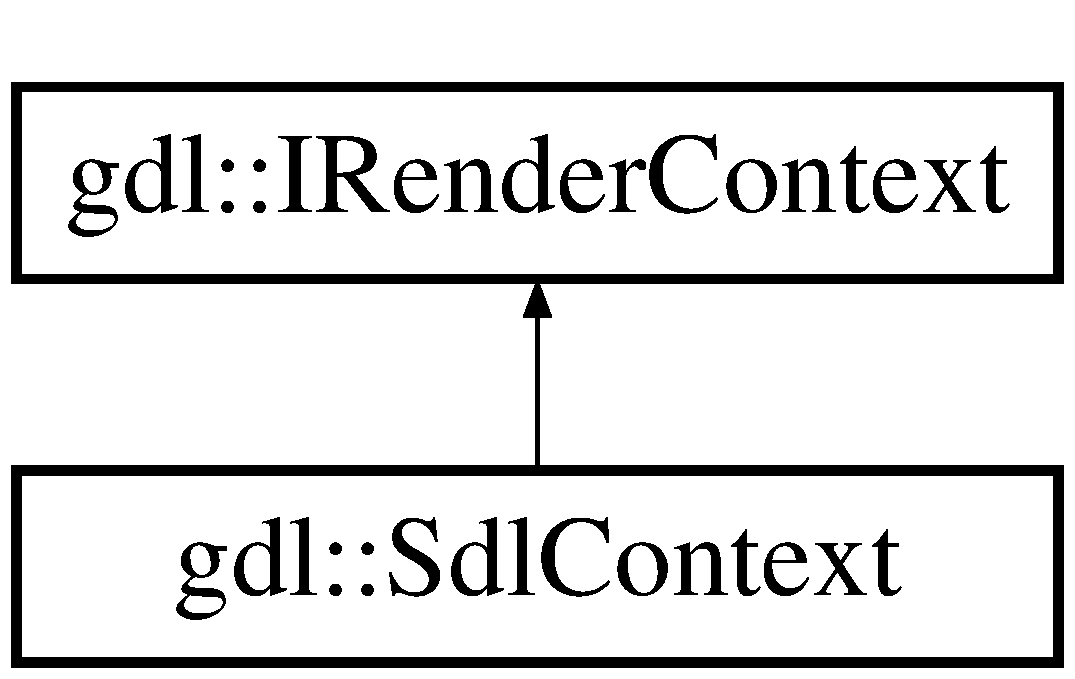
\includegraphics[height=2.000000cm]{classgdl_1_1_sdl_context}
\end{center}
\end{figure}
\subsection*{Public Member Functions}
\begin{DoxyCompactItemize}
\item 
virtual bool \hyperlink{classgdl_1_1_sdl_context_a317e2f02518809a4ff1d4ec381cf29a2}{start} (unsigned int swidth, unsigned int sheight, const std\-::string \&name, int init\-Flags=S\-D\-L\-\_\-\-I\-N\-I\-T\-\_\-\-V\-I\-D\-E\-O, int windows\-Flags=S\-D\-L\-\_\-\-W\-I\-N\-D\-O\-W\-\_\-\-O\-P\-E\-N\-G\-L)
\begin{DoxyCompactList}\small\item\em Start the context, create a window. \end{DoxyCompactList}\item 
virtual void \hyperlink{classgdl_1_1_sdl_context_a899be84a90438d59547155e4aecc2c87}{update\-Inputs} (\hyperlink{classgdl_1_1_input}{Input} \&input) const 
\begin{DoxyCompactList}\small\item\em Update the inputs. \end{DoxyCompactList}\item 
virtual void \hyperlink{classgdl_1_1_sdl_context_aec8807a2f1b9ca64c880286f1046ad2a}{update\-Clock} (\hyperlink{classgdl_1_1_clock}{Clock} \&clock) const 
\begin{DoxyCompactList}\small\item\em Update the game clock. \end{DoxyCompactList}\item 
\hypertarget{classgdl_1_1_sdl_context_a107b456e3df4727c6c32fff36f45faa7}{virtual void \hyperlink{classgdl_1_1_sdl_context_a107b456e3df4727c6c32fff36f45faa7}{flush} () const }\label{classgdl_1_1_sdl_context_a107b456e3df4727c6c32fff36f45faa7}

\begin{DoxyCompactList}\small\item\em Flush the screen to show what has been drawn. (Just call S\-D\-L\-\_\-\-G\-L\-\_\-\-Swap\-Window). \end{DoxyCompactList}\item 
\hypertarget{classgdl_1_1_sdl_context_a02007ea70c7e5a60048c1bb5812b48b6}{virtual void \hyperlink{classgdl_1_1_sdl_context_a02007ea70c7e5a60048c1bb5812b48b6}{stop} () const }\label{classgdl_1_1_sdl_context_a02007ea70c7e5a60048c1bb5812b48b6}

\begin{DoxyCompactList}\small\item\em Close the context and the window. \end{DoxyCompactList}\end{DoxyCompactItemize}
\subsection*{Protected Attributes}
\begin{DoxyCompactItemize}
\item 
\hypertarget{classgdl_1_1_sdl_context_a3c298835a8a3e236d389efeb6c1d3303}{S\-D\-L\-\_\-\-Window $\ast$ \hyperlink{classgdl_1_1_sdl_context_a3c298835a8a3e236d389efeb6c1d3303}{\-\_\-window}}\label{classgdl_1_1_sdl_context_a3c298835a8a3e236d389efeb6c1d3303}

\begin{DoxyCompactList}\small\item\em The S\-D\-L window object. \end{DoxyCompactList}\item 
\hypertarget{classgdl_1_1_sdl_context_a8a997eff1d38bc784ee95ce76db93359}{S\-D\-L\-\_\-\-G\-L\-Context \hyperlink{classgdl_1_1_sdl_context_a8a997eff1d38bc784ee95ce76db93359}{\-\_\-gl\-Context}}\label{classgdl_1_1_sdl_context_a8a997eff1d38bc784ee95ce76db93359}

\begin{DoxyCompactList}\small\item\em The S\-D\-L Open\-G\-L context object. \end{DoxyCompactList}\end{DoxyCompactItemize}


\subsection{Detailed Description}
Class for an Sdl Context. 

\subsection{Member Function Documentation}
\hypertarget{classgdl_1_1_sdl_context_a317e2f02518809a4ff1d4ec381cf29a2}{\index{gdl\-::\-Sdl\-Context@{gdl\-::\-Sdl\-Context}!start@{start}}
\index{start@{start}!gdl::SdlContext@{gdl\-::\-Sdl\-Context}}
\subsubsection[{start}]{\setlength{\rightskip}{0pt plus 5cm}bool gdl\-::\-Sdl\-Context\-::start (
\begin{DoxyParamCaption}
\item[{unsigned int}]{swidth, }
\item[{unsigned int}]{sheight, }
\item[{const std\-::string \&}]{name, }
\item[{int}]{init\-Flags = {\ttfamily SDL\-\_\-INIT\-\_\-VIDEO}, }
\item[{int}]{windows\-Flags = {\ttfamily SDL\-\_\-WINDOW\-\_\-OPENGL}}
\end{DoxyParamCaption}
)\hspace{0.3cm}{\ttfamily [virtual]}}}\label{classgdl_1_1_sdl_context_a317e2f02518809a4ff1d4ec381cf29a2}


Start the context, create a window. 


\begin{DoxyParams}{Parameters}
{\em swidth} & The width of the window to create. \\
\hline
{\em sheight} & The height of the window to create. \\
\hline
{\em name} & The name of the window. \\
\hline
{\em init\-Flags} & Flags passed to S\-D\-L\-\_\-\-Init. \\
\hline
{\em windows\-Flags} & Flags passed to S\-D\-L\-\_\-\-Create\-Window. \\
\hline
\end{DoxyParams}
\begin{DoxyReturn}{Returns}
False if the context creation has failed. 
\end{DoxyReturn}


Implements \hyperlink{classgdl_1_1_i_render_context}{gdl\-::\-I\-Render\-Context}.

\hypertarget{classgdl_1_1_sdl_context_aec8807a2f1b9ca64c880286f1046ad2a}{\index{gdl\-::\-Sdl\-Context@{gdl\-::\-Sdl\-Context}!update\-Clock@{update\-Clock}}
\index{update\-Clock@{update\-Clock}!gdl::SdlContext@{gdl\-::\-Sdl\-Context}}
\subsubsection[{update\-Clock}]{\setlength{\rightskip}{0pt plus 5cm}void gdl\-::\-Sdl\-Context\-::update\-Clock (
\begin{DoxyParamCaption}
\item[{{\bf Clock} \&}]{clock}
\end{DoxyParamCaption}
) const\hspace{0.3cm}{\ttfamily [virtual]}}}\label{classgdl_1_1_sdl_context_aec8807a2f1b9ca64c880286f1046ad2a}


Update the game clock. 


\begin{DoxyParams}{Parameters}
{\em input} & The clock object to update. \\
\hline
\end{DoxyParams}


Implements \hyperlink{classgdl_1_1_i_render_context}{gdl\-::\-I\-Render\-Context}.

\hypertarget{classgdl_1_1_sdl_context_a899be84a90438d59547155e4aecc2c87}{\index{gdl\-::\-Sdl\-Context@{gdl\-::\-Sdl\-Context}!update\-Inputs@{update\-Inputs}}
\index{update\-Inputs@{update\-Inputs}!gdl::SdlContext@{gdl\-::\-Sdl\-Context}}
\subsubsection[{update\-Inputs}]{\setlength{\rightskip}{0pt plus 5cm}void gdl\-::\-Sdl\-Context\-::update\-Inputs (
\begin{DoxyParamCaption}
\item[{{\bf Input} \&}]{input}
\end{DoxyParamCaption}
) const\hspace{0.3cm}{\ttfamily [virtual]}}}\label{classgdl_1_1_sdl_context_a899be84a90438d59547155e4aecc2c87}


Update the inputs. 


\begin{DoxyParams}{Parameters}
{\em input} & The input object to fill. \\
\hline
\end{DoxyParams}


Implements \hyperlink{classgdl_1_1_i_render_context}{gdl\-::\-I\-Render\-Context}.



The documentation for this class was generated from the following files\-:\begin{DoxyCompactItemize}
\item 
includes/Sdl\-Context.\-hh\item 
sources/Sdl\-Context.\-cpp\end{DoxyCompactItemize}

\hypertarget{classgdl_1_1_texture}{\section{gdl\-:\-:Texture Class Reference}
\label{classgdl_1_1_texture}\index{gdl\-::\-Texture@{gdl\-::\-Texture}}
}


Class representing an Open\-G\-L texture.  




{\ttfamily \#include $<$Texture.\-hh$>$}

\subsection*{Public Member Functions}
\begin{DoxyCompactItemize}
\item 
\hypertarget{classgdl_1_1_texture_a2d010f85c81be8c5b19cf7b4f0ae1af0}{{\bfseries Texture} (\hyperlink{classgdl_1_1_texture}{Texture} const \&o)}\label{classgdl_1_1_texture_a2d010f85c81be8c5b19cf7b4f0ae1af0}

\item 
bool \hyperlink{classgdl_1_1_texture_ada7dffc24ec794f7cc5a5a26dc0261fc}{load} (const std\-::string \&path, bool gen\-Mimaps=false)
\begin{DoxyCompactList}\small\item\em Load a T\-G\-A file. \end{DoxyCompactList}\item 
G\-Luint \hyperlink{classgdl_1_1_texture_a1954740f65f3e9265d6f4506ec75f4c2}{get\-Id} () const 
\begin{DoxyCompactList}\small\item\em Returns the Open\-G\-L texture I\-D. \end{DoxyCompactList}\item 
\hypertarget{classgdl_1_1_texture_a5b628612f89e1fc67a28085158236d9c}{void \hyperlink{classgdl_1_1_texture_a5b628612f89e1fc67a28085158236d9c}{bind} () const }\label{classgdl_1_1_texture_a5b628612f89e1fc67a28085158236d9c}

\begin{DoxyCompactList}\small\item\em Bind the texture as the current used texture (call gl\-Bind\-Texture). \end{DoxyCompactList}\item 
G\-Luint \hyperlink{classgdl_1_1_texture_a932fca1cf9da4570df0591ae2272f545}{get\-Width} () const 
\item 
G\-Luint \hyperlink{classgdl_1_1_texture_a7ffaf22e021293cab2a856c2ec795dca}{get\-Height} () const 
\item 
\hypertarget{classgdl_1_1_texture_afc8d4545507f62b5273f938dce5dfeba}{\hyperlink{classgdl_1_1_texture}{Texture} \& {\bfseries operator=} (\hyperlink{classgdl_1_1_texture}{Texture} const \&o)}\label{classgdl_1_1_texture_afc8d4545507f62b5273f938dce5dfeba}

\end{DoxyCompactItemize}
\subsection*{Protected Attributes}
\begin{DoxyCompactItemize}
\item 
\hypertarget{classgdl_1_1_texture_a649311ec115dcd70df025714d52f887e}{G\-Luint {\bfseries \-\_\-width}}\label{classgdl_1_1_texture_a649311ec115dcd70df025714d52f887e}

\item 
\hypertarget{classgdl_1_1_texture_ad016a8f5410560f0ac2498eb75ba7570}{G\-Luint {\bfseries \-\_\-height}}\label{classgdl_1_1_texture_ad016a8f5410560f0ac2498eb75ba7570}

\item 
\hypertarget{classgdl_1_1_texture_ad583257567501c6c9f58b943c03cde68}{G\-Luint {\bfseries \-\_\-id}}\label{classgdl_1_1_texture_ad583257567501c6c9f58b943c03cde68}

\end{DoxyCompactItemize}


\subsection{Detailed Description}
Class representing an Open\-G\-L texture. 

\subsection{Member Function Documentation}
\hypertarget{classgdl_1_1_texture_a7ffaf22e021293cab2a856c2ec795dca}{\index{gdl\-::\-Texture@{gdl\-::\-Texture}!get\-Height@{get\-Height}}
\index{get\-Height@{get\-Height}!gdl::Texture@{gdl\-::\-Texture}}
\subsubsection[{get\-Height}]{\setlength{\rightskip}{0pt plus 5cm}G\-Luint gdl\-::\-Texture\-::get\-Height (
\begin{DoxyParamCaption}
{}
\end{DoxyParamCaption}
) const}}\label{classgdl_1_1_texture_a7ffaf22e021293cab2a856c2ec795dca}
\begin{DoxyReturn}{Returns}
The height of the texture 
\end{DoxyReturn}
\hypertarget{classgdl_1_1_texture_a1954740f65f3e9265d6f4506ec75f4c2}{\index{gdl\-::\-Texture@{gdl\-::\-Texture}!get\-Id@{get\-Id}}
\index{get\-Id@{get\-Id}!gdl::Texture@{gdl\-::\-Texture}}
\subsubsection[{get\-Id}]{\setlength{\rightskip}{0pt plus 5cm}G\-Luint gdl\-::\-Texture\-::get\-Id (
\begin{DoxyParamCaption}
{}
\end{DoxyParamCaption}
) const}}\label{classgdl_1_1_texture_a1954740f65f3e9265d6f4506ec75f4c2}


Returns the Open\-G\-L texture I\-D. 

\begin{DoxyReturn}{Returns}
The Open\-G\-L texture Id. 
\end{DoxyReturn}
\hypertarget{classgdl_1_1_texture_a932fca1cf9da4570df0591ae2272f545}{\index{gdl\-::\-Texture@{gdl\-::\-Texture}!get\-Width@{get\-Width}}
\index{get\-Width@{get\-Width}!gdl::Texture@{gdl\-::\-Texture}}
\subsubsection[{get\-Width}]{\setlength{\rightskip}{0pt plus 5cm}G\-Luint gdl\-::\-Texture\-::get\-Width (
\begin{DoxyParamCaption}
{}
\end{DoxyParamCaption}
) const}}\label{classgdl_1_1_texture_a932fca1cf9da4570df0591ae2272f545}
\begin{DoxyReturn}{Returns}
The width of the texture 
\end{DoxyReturn}
\hypertarget{classgdl_1_1_texture_ada7dffc24ec794f7cc5a5a26dc0261fc}{\index{gdl\-::\-Texture@{gdl\-::\-Texture}!load@{load}}
\index{load@{load}!gdl::Texture@{gdl\-::\-Texture}}
\subsubsection[{load}]{\setlength{\rightskip}{0pt plus 5cm}bool gdl\-::\-Texture\-::load (
\begin{DoxyParamCaption}
\item[{const std\-::string \&}]{path, }
\item[{bool}]{gen\-Mimaps = {\ttfamily false}}
\end{DoxyParamCaption}
)}}\label{classgdl_1_1_texture_ada7dffc24ec794f7cc5a5a26dc0261fc}


Load a T\-G\-A file. 


\begin{DoxyParams}{Parameters}
{\em path} & The path of the T\-G\-A file. \\
\hline
{\em gen\-Mipmaps} & If true, mipmaps will be generated and used as minfilter for this texture. \\
\hline
\end{DoxyParams}
\begin{DoxyReturn}{Returns}
False if the load has failed. 
\end{DoxyReturn}


The documentation for this class was generated from the following files\-:\begin{DoxyCompactItemize}
\item 
includes/Texture.\-hh\item 
sources/Texture.\-cpp\end{DoxyCompactItemize}

%--- End generated contents ---

% Index
\newpage
\phantomsection
\addcontentsline{toc}{chapter}{Index}
\printindex

\end{document}
